\documentclass{cmspaper}
%
% LaTeX packages
%
\usepackage{graphicx}
\usepackage{epic,rotating,epsfig}
\usepackage{amssymb}
\usepackage{amsmath}
\usepackage{pstricks,pst-grad}
\usepackage{subfigure}
\usepackage{multirow} 
\usepackage{subfigure}
\usepackage{lineno}
%\usepackage{feynmf}
%\usepackage{xcolor}
\usepackage{url} 
\usepackage{amssymb} 
\usepackage{textcomp} 
\usepackage{hyperref} 
\usepackage{graphicx}
\usepackage[T1]{fontenc}
\usepackage[latin1]{inputenc}
\setcounter{secnumdepth}{3}
\setcounter{tocdepth}{3}
\usepackage{amsfonts}
\usepackage{multirow}
\usepackage{float}

\def\cm{\hbox{$\;\hbox{\rm cm}$}}
\def\eV{\hbox{$\;\hbox{\rm eV}$}}
\def\GeV{\hbox{$\;\hbox{\rm GeV}$}}
\def\MeV{\hbox{$\;\hbox{\rm MeV}$}}
\def\TeV{\hbox{$\;\hbox{\rm TeV}$}}
\newcommand{\Zee}{\mbox{$\rm Z\rightarrow\rm e^{+} \rm e^{-}$}}
\newcommand{\Wenu}{\mbox{$\rm W\rightarrow\rm e \rm \nu$}}
\newcommand{\Z}{\mbox{$\rm Z$}}
\newcommand{\W}{\mbox{$\rm W$}}
\newcommand{\TeVcc}{\ensuremath{\,\mathrm{Te\kern -0.1em V\!/c}^2}}
\newcommand{\GeVcc}{\ensuremath{\,\mathrm{~Ge\kern -0.1em V\!/c}^2}}
\newcommand{\MeVcc}{\ensuremath{\,\mathrm{Me\kern -0.1em V\!/c}^2}}
\newcommand{\GeVc}{\ensuremath{\mathrm{~Ge\kern -0.1em V}\!/c}}
\newcommand{\nanob}{\mbox{{\rm ~nb}}}
\newcommand{\fb}{\ensuremath{\mathrm{fb}}}
\newcommand{\pb}{\ensuremath{\mathrm{pb}}}
\newcommand{\ifb}{\ensuremath{\mathrm{fb^{-1}}}}
\newcommand{\ipb}{\ensuremath{\mathrm{pb^{-1}}}}
\newcommand{\Hmu}{\ensuremath{\mathrm{H}\to\mathrm{ZZ^{(\ast)}}\to4\mu}}
\newcommand{\HZe}{\ensuremath{\mathrm{H}\to\mathrm{ZZ^{(\ast)}}\to4e}}
\newcommand{\HWe}{\ensuremath{\mathrm{H}\to\mathrm{WW^{(\ast)}}\to e\nu e\nu }}
\newcommand{\mmu}{\ensuremath{\mathrm{m_{4\mu}}}}
\newcommand{\mH}{\ensuremath{m_{\mathrm{H}}}}
\newcommand{\Lumi}{\ensuremath{{\cal L}}}
\newcommand{\lnQ}{\ensuremath{\mathrm{ln}(Q)}}
\newcommand{\mlnQ}{\ensuremath{-2\,\mathrm{ln}(Q)}}
\newcommand{\LS}{\ensuremath{{\cal L}(S)}}
\newcommand{\LB}{\ensuremath{{\cal L}(B)}}
\newcommand{\LSB}{\ensuremath{{\cal L}(S+B)}}
\newcommand{\mZ}{\ensuremath{m_\mathrm{Z}}}
\newcommand{\Zbb}{\ensuremath{(Z/\gamma^*){\mathrm{b\bar{b}}}}}
\newcommand{\ttbar}{\ensuremath{\mathrm{t\bar{t}}}}
\newcommand{\ZZ}{\ensuremath{\mathrm{Z/\gamma^*Z/\gamma^*}}}
\newcommand{\Zgam}{\ensuremath{\mathrm{Z/\gamma^*}}}
\newcommand{\mumu}{\ensuremath{\mathrm{\mu^+\mu^-}}}
\newcommand{\lsim}{\raisebox{-1.5mm}{$\:\stackrel{\textstyle{<}}{\textstyle{\sim}}\:$}}
\newcommand{\gsim}{\raisebox{-1.5mm}{$\:\stackrel{\textstyle{>}}{\textstyle{\sim}}\:$}}
\newcommand{\et}{\mbox{$\mathrm{E_{T}}$}}
\newcommand{\met}{\mbox{$\mathrm{E\!\!\!/_{T}}$}}
\newcommand{\etsc}{\mbox{$\mathrm{E_{T}^{SC}}$}}
\newcommand{\dr}{\mbox{$\mathrm{\Delta R}$}}

\newcommand{\dPhiIn}{\ensuremath{\mathrm{\Delta\phi_{in}}}}
\newcommand{\dEtaIn}{\ensuremath{\Delta\eta_{\mathrm{in}}}}
\newcommand{\hoe}{\ensuremath{\mathrm{H}/\mathrm{E}}}
\newcommand{\sigmaIEtaIEta}{\ensuremath{\sigma_{\mathrm{i}\eta\mathrm{i}\eta}}}
\newcommand{\sigmaEtaEta}{\ensuremath{\sigma_{\eta\eta}}}
\newcommand{\eTwoByFive}{\ensuremath{\mathrm{E}^{2\times5}/\mathrm{E}^{5\times5}}}
\newcommand{\eOneByFive}{\ensuremath{\mathrm{E}^{1\times5}/\mathrm{E}^{5\times5}}}
\newcommand{\pin}{\ensuremath{\mathrm{p_{in}}}}
\newcommand{\pout}{\ensuremath{\mathrm{p_{out}}}}
\newcommand{\pt}{\ensuremath{\mathrm{p_{T}}}}
\newcommand{\eseedpin}{\ensuremath{\mathrm{E_{seed}}/\mathrm{p_{in}}}}
\newcommand{\eseedpout}{\ensuremath{\mathrm{E_{seed}}/\mathrm{p_{out}}}}
\newcommand{\epin}{\ensuremath{\mathrm{E}/\mathrm{p_{in}}}}

%

%==========================================================

\begin{document}
\begin{titlepage}
\internalnote{2010/xxx}
\date{\today}
\title{Electron GSF Tracking Commissioning with first LHC Data}
\begin{Authlist}

%M.~Sani\Aref{a}, 
 
%\Instfoot{a}{a) University of California, San Diego} 

\end{Authlist}
\begin{abstract}
The first LHC collisions at center of mass energies of 900 GeV and 2.36 TeV were recorded by the CMS
detector in December 2009. 
The Category Based Electron Identification selection relies on the
fBrem variable measurement to categorize the Electrons, hence on the
quality of the GSF Tracking.
It is then of vital importance its commissioning with the first
recorded data.
In this analysis we perform a full comparison of GSF track variables as reconstructed in data and 
in the simulated 900 GeV Monte Carlo events focusing on the relevant
observables used in Electron Identification selection.

\end{abstract}                          

\end{titlepage}

\clearpage 
\tableofcontents
\clearpage

\linenumbers

\newpage

\pagenumbering{arabic}

\section{Introduction}\label{sec:Introduction}

The bremsstrahlung energy loss distribution of electrons propagating in matter is highly non-Gaussian.
Since the Kalman filter relies solely on Gaussian probability
density functions, it is not necessarily the optimal reconstruction
algorithm for electron tracks. 
To better model the energy loss a Gaussian mixture rather than a
single Gaussian can be used and this is implemented in the
Gaussian-sum filter (GSF) algorithm. 

The GSF algorithm has been developed in the CMS reconstruction
software and heavily used for electron reconstruction in the CMS
detector. The GSF leads to trajectory states for each measurement
point. In particular the momentum measurements at the inner ($\pin$) and
outer ($\pout$) state are available making possible to give an estimate
of the amount of energy loss in the Tracker ($\fbrem = (\pin-\pout)/\pin$).

The Category Based Electron Identification selection relies on the
$\fbrem$ measurement to categorize the Electrons and to try to separate
them from fakes.
The commissioning of the GSF Tracking is therefore crucial to validate
the Electron Identification selection.

The first collisions at CMS were recorded in December 2009 at energies of $\sqrt{s} = 900 \GeV$ and $2.36 \TeV$. 
The reconstructed electrons in this data have been studied extensively to commission 
the electron reconstruction and identification. Unfortunately the number of electron candidates produced
in these collisions is low and to better commission pure tracking quantities we have performed a full
re-reconstruction of the GSF tracks using standard tracking seeds. 
This allowed us to greatly increase the
available statistic.

In this note we focus on GSF track comparison between data and Monte Carlo.

\section{Data and MC Samples}\label{sec:Samples}

The latest available data reprocessing, labelled as January $29^{\mathrm{th}}$, has
been used in this analysis.
The events have been analyzed using the \verb=CMSSW_3_3_6_patch4=
version of the CMS reconstruction software.
The data have been then compared with the Monte Carlo prediction obtained from the simulated 900 GeV 
Minimum Bias events:\\
/MinBias/Summer09-STARTUP3X\_V8P\_900GeV-v1/GEN-SIM-RECO. 

In reprocessing the data the standard parameters for electron
reconstruction have been used.
Also the collection of GSF tracks, that we have analyzed, have been reconstructed starting from the 
seed collection used for general CTF tracking (\verb=newCombinedSeeds=).
Since this study mainly concerns electron properties, the parameters of the GSF Tracking 
algorithm (pattern recognition and fitting) have been set to the default values used in the 
standard electron reconstruction.

\section{Selections}\label{sec:Selections}

\subsection{Event Selection}
The available data statistic has been selected by run and lumi-section according to the
particular conditions of the detector during the data taking. 
For the GSF Tracking study we have selected events from collisions at 900 GeV
center of mass energy, requiring that the CMS magnetic field was 3.8~T. 

Among the selected good runs we have also applied the following selection on each event:
\begin{itemize}
\item BPTX 
\item L1 technical trigger bit 34 (BSC ``OR'') fired and not 36, 37, 38, 39 (beam halo gas veto),
\item hltPhysicsDeclared on
\item at least one hit with 2 GeV energy in both HF,
\item at least one vertex in the event with $\d0$ < 2~cm, |z|<15~cm, with at least 4 degrees of freedom,
\item in events with more than 10 reconstructed tracks at least 25\%
  of them must be ``high purity''. 
\end{itemize}

These selections lead to the run/lumi-section list shown in Table~\ref{tab:run lumis}.

\begin{table}[htbp]
\begin{center}
\begin{tabular}{|l|l|c|}
\hline
Run  & Lumisec & \multicolumn{1}{l|}{Events} \\ \hline
123815 & 8-9999 & 427 \\ \hline
123818 & 2-42 & 1075 \\ \hline
123906 & 18-28 & 186 \\ \hline
123908 & 2-12 & 102 \\ \hline
124006 & 7-9999 & 65 \\ \hline
124008 & 1-1 & 46 \\ \hline
124009 & 1-68 & 10736 \\ \hline
124020 & 12-94 & 17579 \\ \hline
124022 & 66-179 & 41341 \\ \hline
124023 & 38-9999 & 35641 \\ \hline
124024 & 2-83 & 29343 \\ \hline
124025 & 5-13 & 2644 \\ \hline
124027 & 24-9999 & 13301 \\ \hline
124030 & 2-9999 & 18514 \\ \hline
 &  & 171000 \\ \hline
\end{tabular}
\caption{List of the good run/lumi-section used in the analysis with the corresponding number of events passing the selection described in the text.}
\label{tab:run lumis}
\end{center}
\end{table}

\subsection{Track Selection}

The study of the GSF track properties has been carried on with a selected set of good tracks.
To separate the badly reconstructed tracks to the good ones with have applied the following criteria:

\begin{itemize}
\item the track has to be at least 7 hits.
\item the track must be qualified ``high purity'' and has to be reconstructed during the 0th and 1st iterations
of iterative tracking procedure (using only pixel triplet and pair seeds). Since this information is not 
directly available for GSF track we have first matched the GSF track to one of the reconstructed CTF tracks and
then we have used the information stored in the CTF. The matching has been done by hits, requiring the
two tracks to have at least 50\% of shared hits (fraction computed on the shortest track).
\end{itemize}

As a cross-check some of the following results have been checked for
the full set of reconstructed tracks also.

\section{Results}\label{sec:Results}

In this section the complete set of results is presented. If not specified the following plots
are normalized to the number of data entries and refer to high purity tracks.

Tab.~\ref{tab:numbers} reports the number of events and tracks used in the analysis, together with the 
number of tracks falling in the different categories. About 67\% of the analyzed tracks passed quality cuts, 
while only few percent (~4\%) of them could not be associated to any reconstructed CTF track. 
Looking more closely to the reconstructed electron candidates it turns out that almost 95\% of them 
has an high purity GSF track.
The Table~\ref{tab:numbers} also shows how the Monte Carlo simulation foresees about 20\% less reconstructed
tracks.

\begin{table}[htbp]
\begin{center}
\begin{tabular}{|c|c|c|c|c|c|c|}
\hline
 & Events & Tracks & \multicolumn{1}{c|}{Tk/evt} & Quality & No High purity & No CTF match \\ \hline
Data & \multicolumn{1}{c|}{171000} & \multicolumn{1}{c|}{1404937} & 8.22 & \multicolumn{1}{c|}{946228} & \multicolumn{1}{c|}{398277} & \multicolumn{1}{c|}{60432} \\ \hline
MC & \multicolumn{1}{c|}{494675} & \multicolumn{1}{c|}{33374188} & 6.82 & \multicolumn{1}{c|}{2393783} & \multicolumn{1}{c|}{868378} & \multicolumn{1}{c|}{116527} \\ \hline
% &  &  & 1.2 &  &  &  \\ \hline
\end{tabular}
\end{center}
\caption{Number of data and minimum bias events analyzed. The table shows the corresponding number of reconstructed GSF Tracks split in different categories.}
\label{tab:numbers}
\end{table}

Fig.~\ref{fig:pt distribution} shows the $\pt$ distribution of the GSF tracks in data and MC. 
The distributions are normalized to the total number of reconstructed GSF tracks in data 
and show an excess of data in the Barrel. The transverse momentum ($\pt$) distributions of GSF
tracks are anyway well reproduced.

\begin{figure}
  \begin{center}
    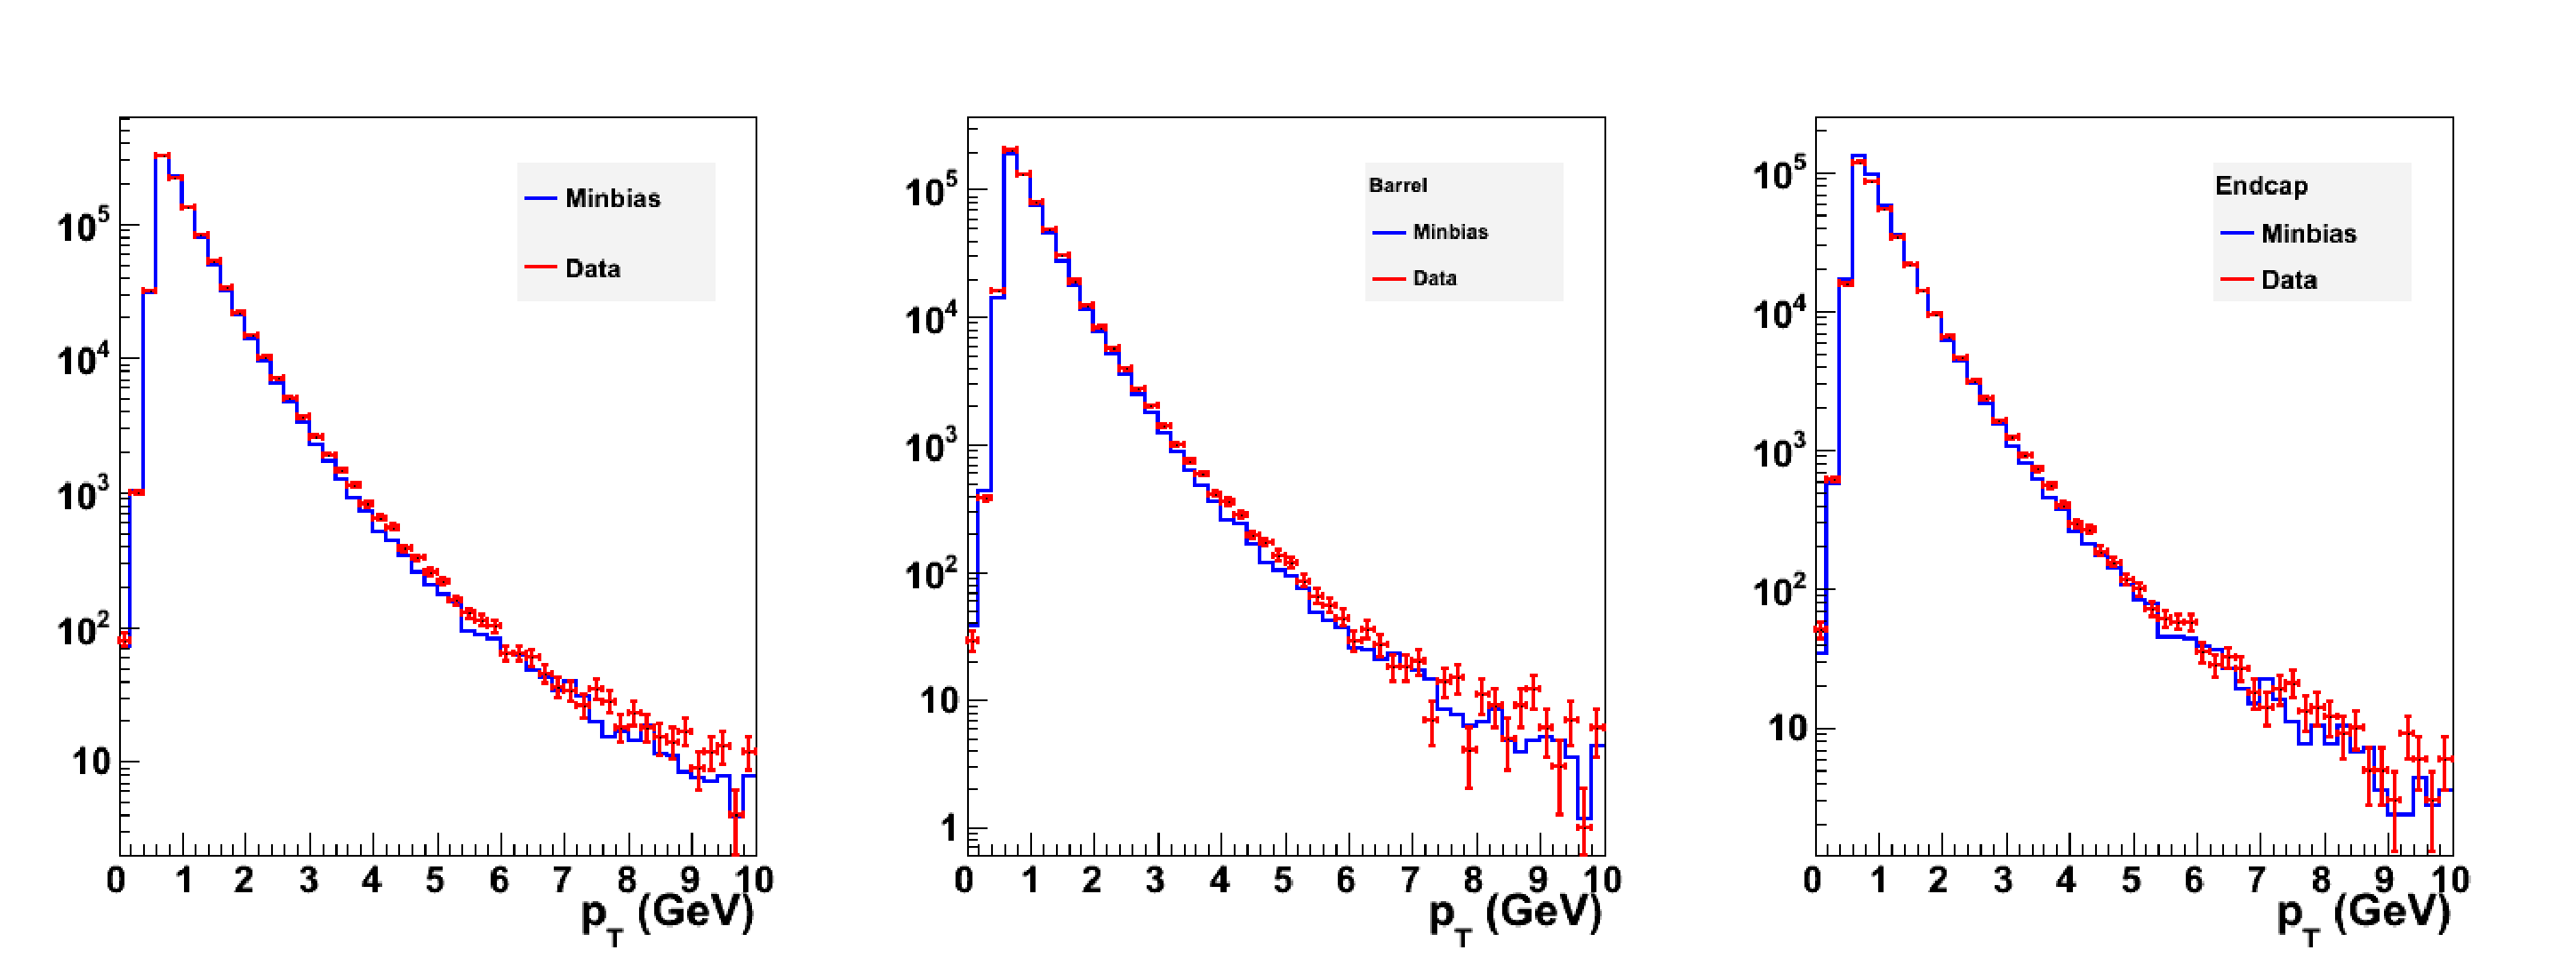
\includegraphics[width=1\textwidth]{Images/gsf_pt_log.eps}
      \caption {Transverse momentum ($\pt$) distribution of GSF tracks in data (points) and MC (histogram). The three plots shows, from left to right, the total distribution, tracks in the barrel and tracks in the Endcap. The three plots are normalized to the total number of reconstructed tracks in data.}
    \label{fig:pt distribution}
  \end{center}
\end{figure}

Fig.~\ref{fig:eta distribution high purity} (a) and (b) show rapidity ($\eta$)
distributions for GSF and CTF high purity tracks. There are some
discrepancies in the high $\eta$ regions in both the distributions. 
The bias is not completely understood but it is introduced by the
quality requirements. If the cut is removed and all the tracks are selected, Fig.~\ref{fig:eta
  distribution high purity} (c), the
agreement between data and MC improves. 
%This last distribution is in good agreement with what observed by the Tracking group.

\begin{figure}
  \begin{center}
    \subfigure[]{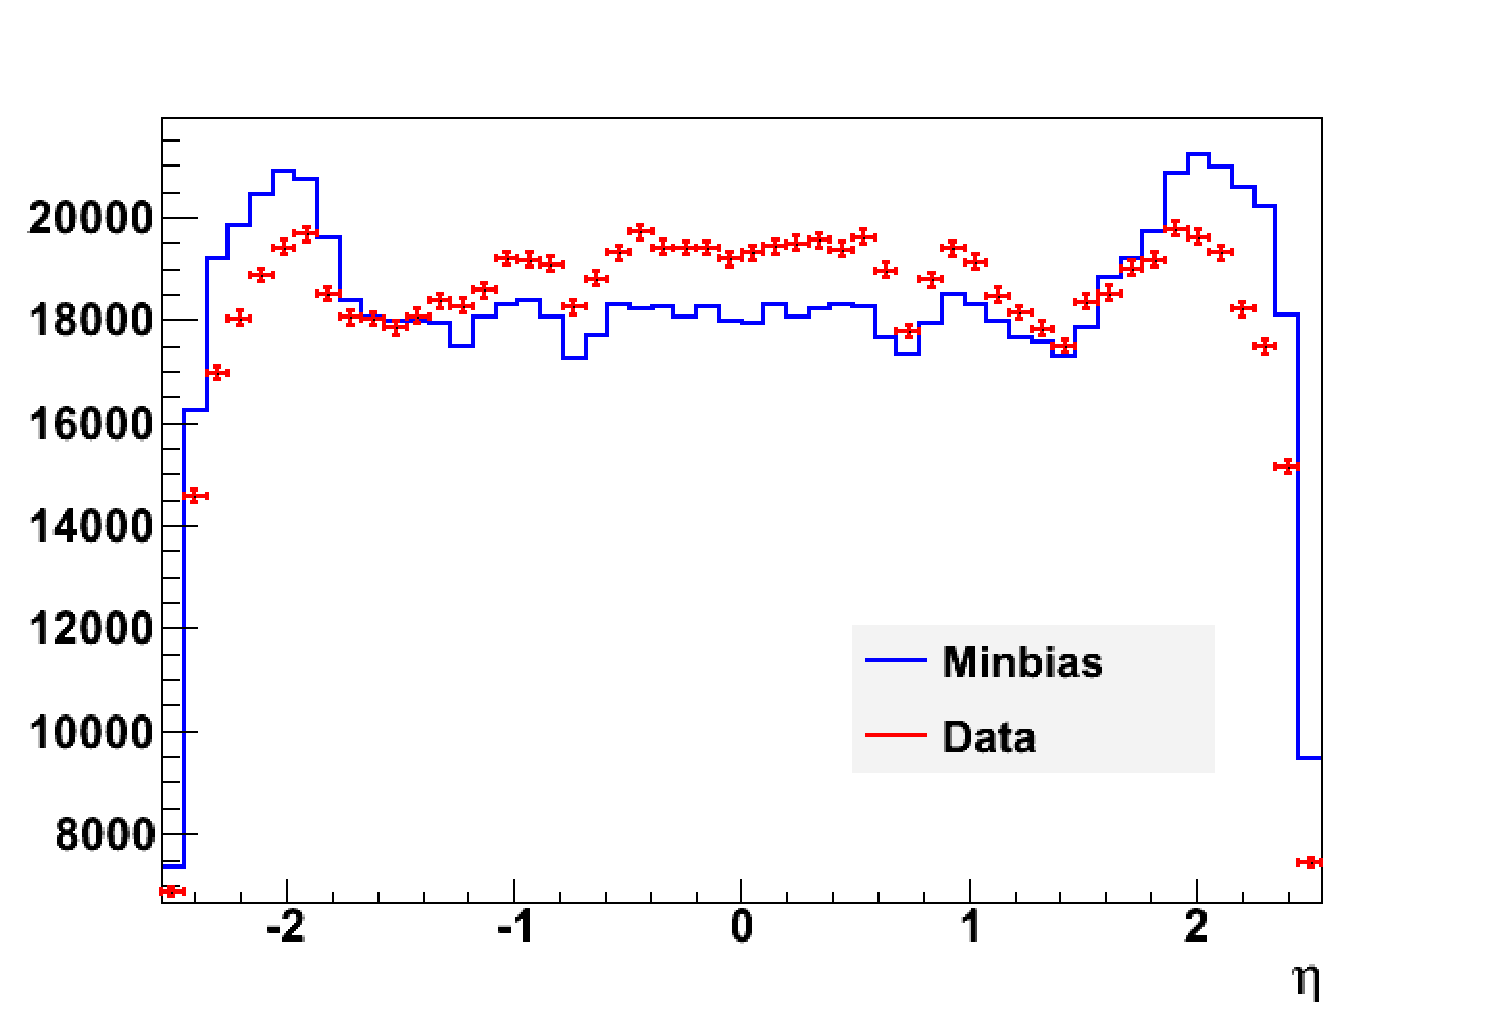
\includegraphics[width=0.45\textwidth]
      {Images/gsf_eta.eps}}
    \subfigure[]{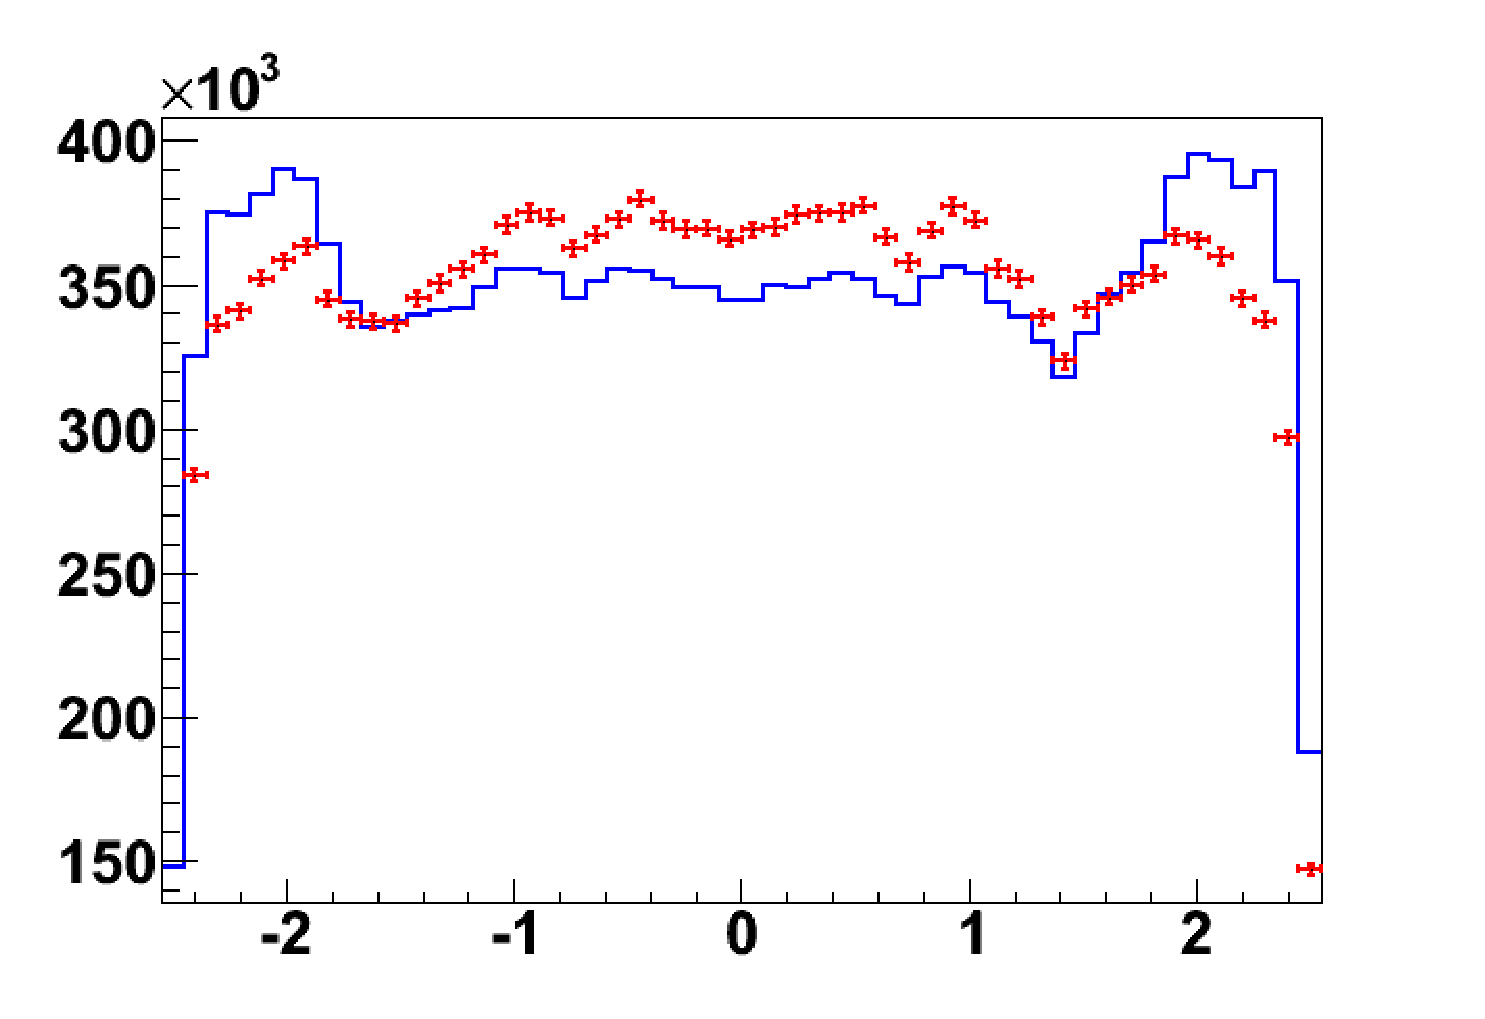
\includegraphics[width=0.45\textwidth]
      {Images/ctf_eta.eps}}
    \subfigure[]{ 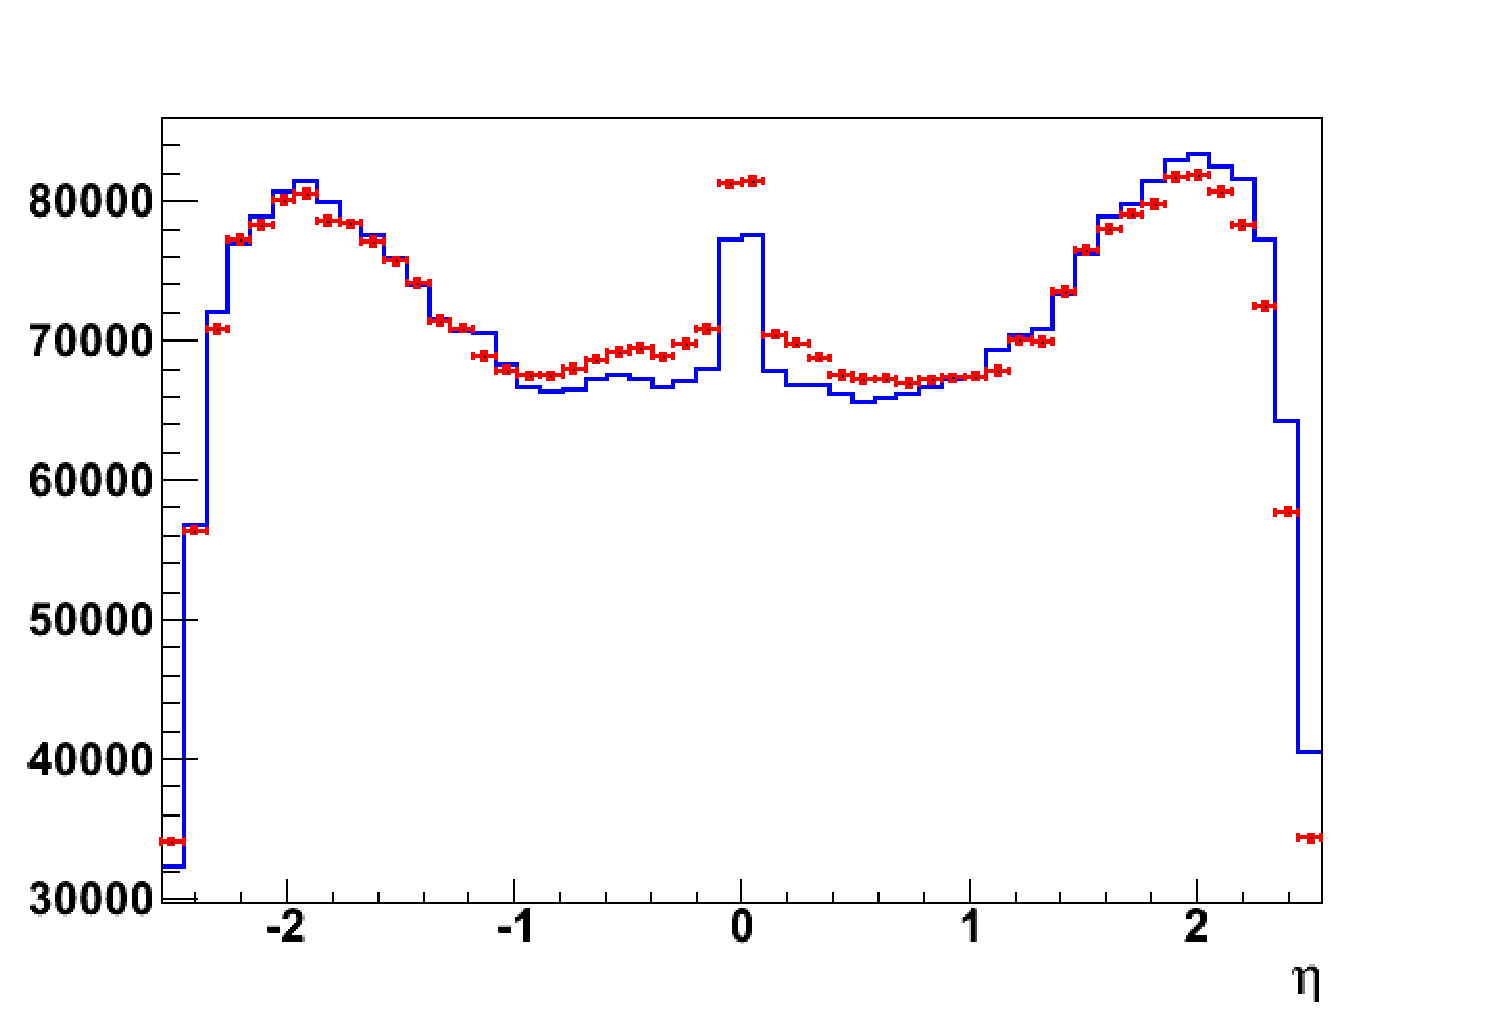
\includegraphics[width=0.45\textwidth]{Images/ctf_eta_all.eps}}
    \caption {$\eta$ distribution of the high purity GSF (a) and CTF (b) Tracks. The $\eta$ distribution of all the tracks is shown in (c). Data are in points, MC in histogram.}
    \label{fig:eta distribution high purity}
  \end{center}
\end{figure}

As already stated the $\fbrem$ variable (defined as $(\pin-\pout)/\pin$)
gives an estimate of the energy loss of an electron indipendently by
the Calorimeter using only the Tracker. This variable is extensively
used in the Category Based Electron Identification so it is important
to check how well it is reproduced by the MC simulation.
Since the large majority of the reconstructed GSF tracks belong to
pions, which doesn't brem, we expect a distribution peaked at 0.

The $\fbrem$ distribution of the GSF tracks has been studied in $\pt$ and $\eta$ bins. Fig.~\ref{fig:fbrem in eta bins} shows the $\fbrem$ distributions in bins of the rapidity.
The agreement between data and MC is very good in the central part of the detector ($|\eta| < 1.0$). Then, as the quantity of
tracker material increases, the peak in data seems to be slightly shifted towards 1 and does not match with the MC expectations.  
In the Endcap the discrepancy is more pronounced.
Fig.~\ref{fig:fbrem in eta bins} shows the $\fbrem$ variable in four $\eta$ bins: two in the barrel and two
in the Endcap. The results for the forward and bakcward sides of the detector are shown separately and no particular asymmetry can be revealed.

\begin{figure}[p]
  \begin{center}
    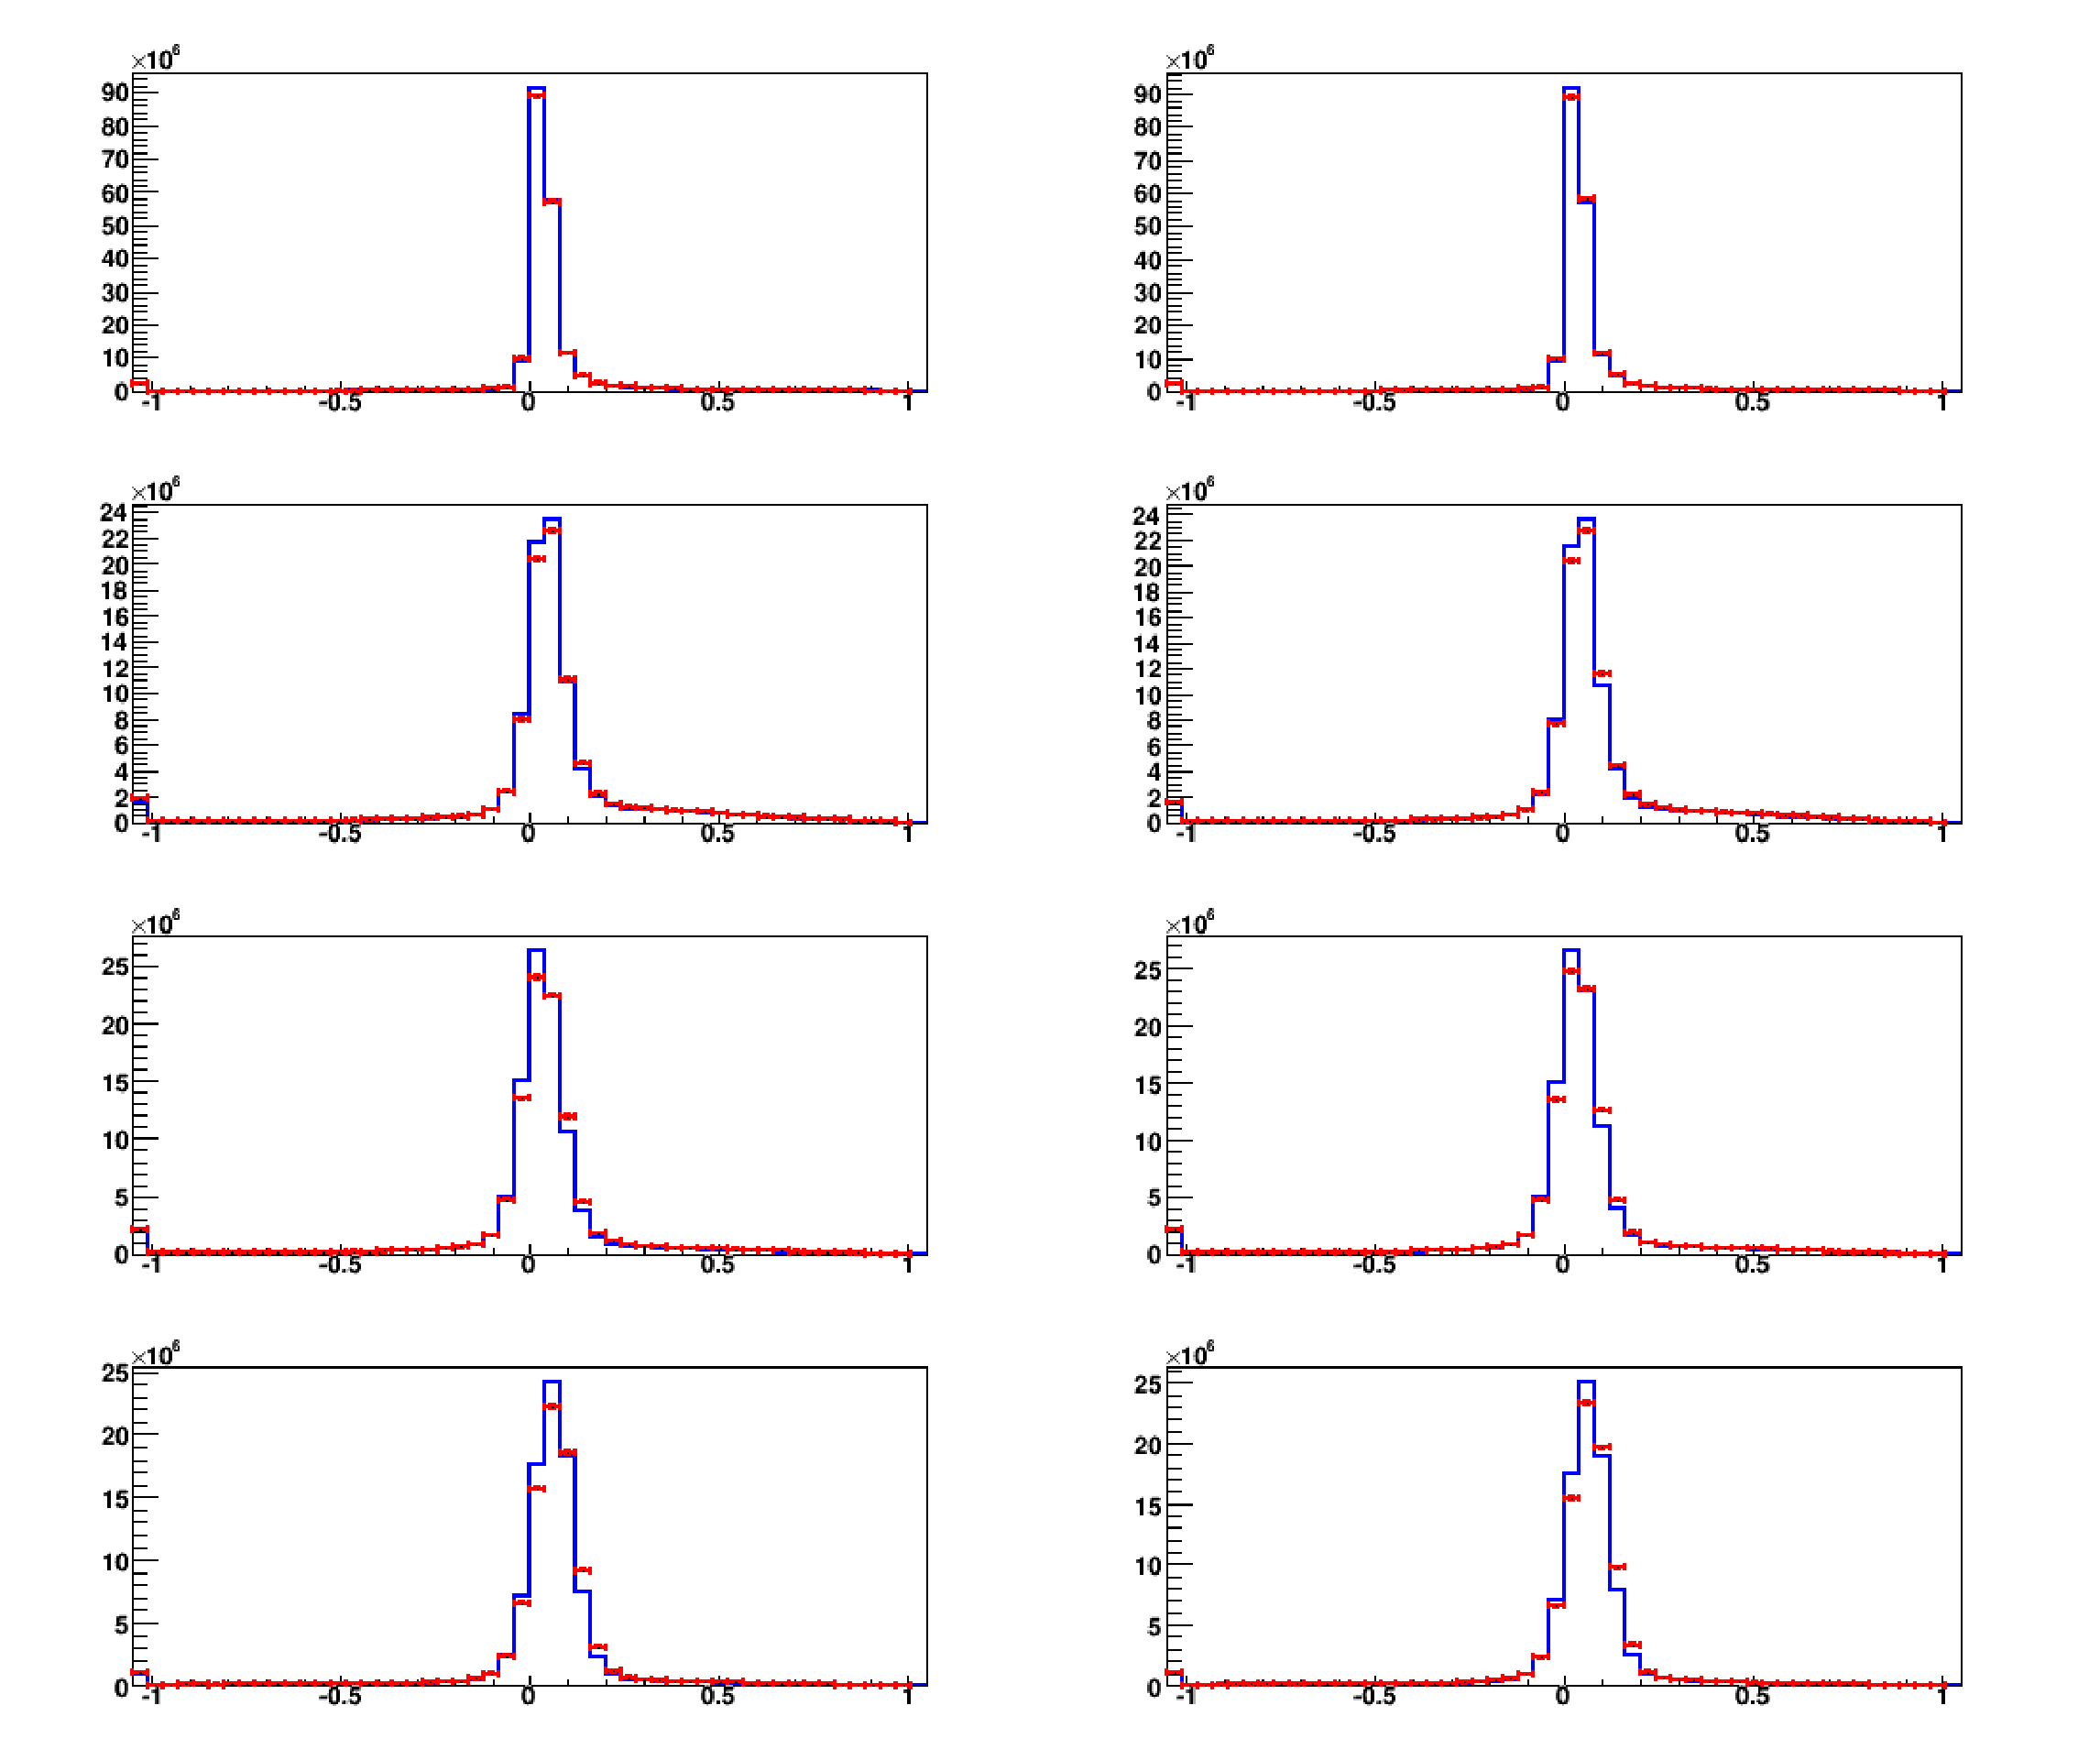
\includegraphics[width=1\textwidth]{Images/fbrem_vs_eta.eps}
    \caption {$\fbrem$ distribution in $\eta$ bins for highpurity GSF Tracks in data (points) and MC (histogram). The four
$\eta$ bins are from top to bottom: $|\eta|$ < 1, $1<|\eta|<1.479$ ,$1.479<|\eta|< 2$, $|\eta| > 2$. Each row shows the distributions for forward and backward sides of the CMS detector.}
    \label{fig:fbrem in eta bins}
  \end{center}
\end{figure}


The fbrem binning in $\pt$ of the GSF track confirms the shift of the peak in the Endcap, showing, at the
same time, no $\pt$ dependence of the effect.
These results are in agreement with what has been seen in the analysis of the electron candidates only.
Fig.~\ref{fig:fbrem in pt bins} reports the results and Fig.~\ref{fig:fbrem tot} shows the total fbrem 
distribution in Barrel and Endcap.

\begin{figure}
  \begin{center}
    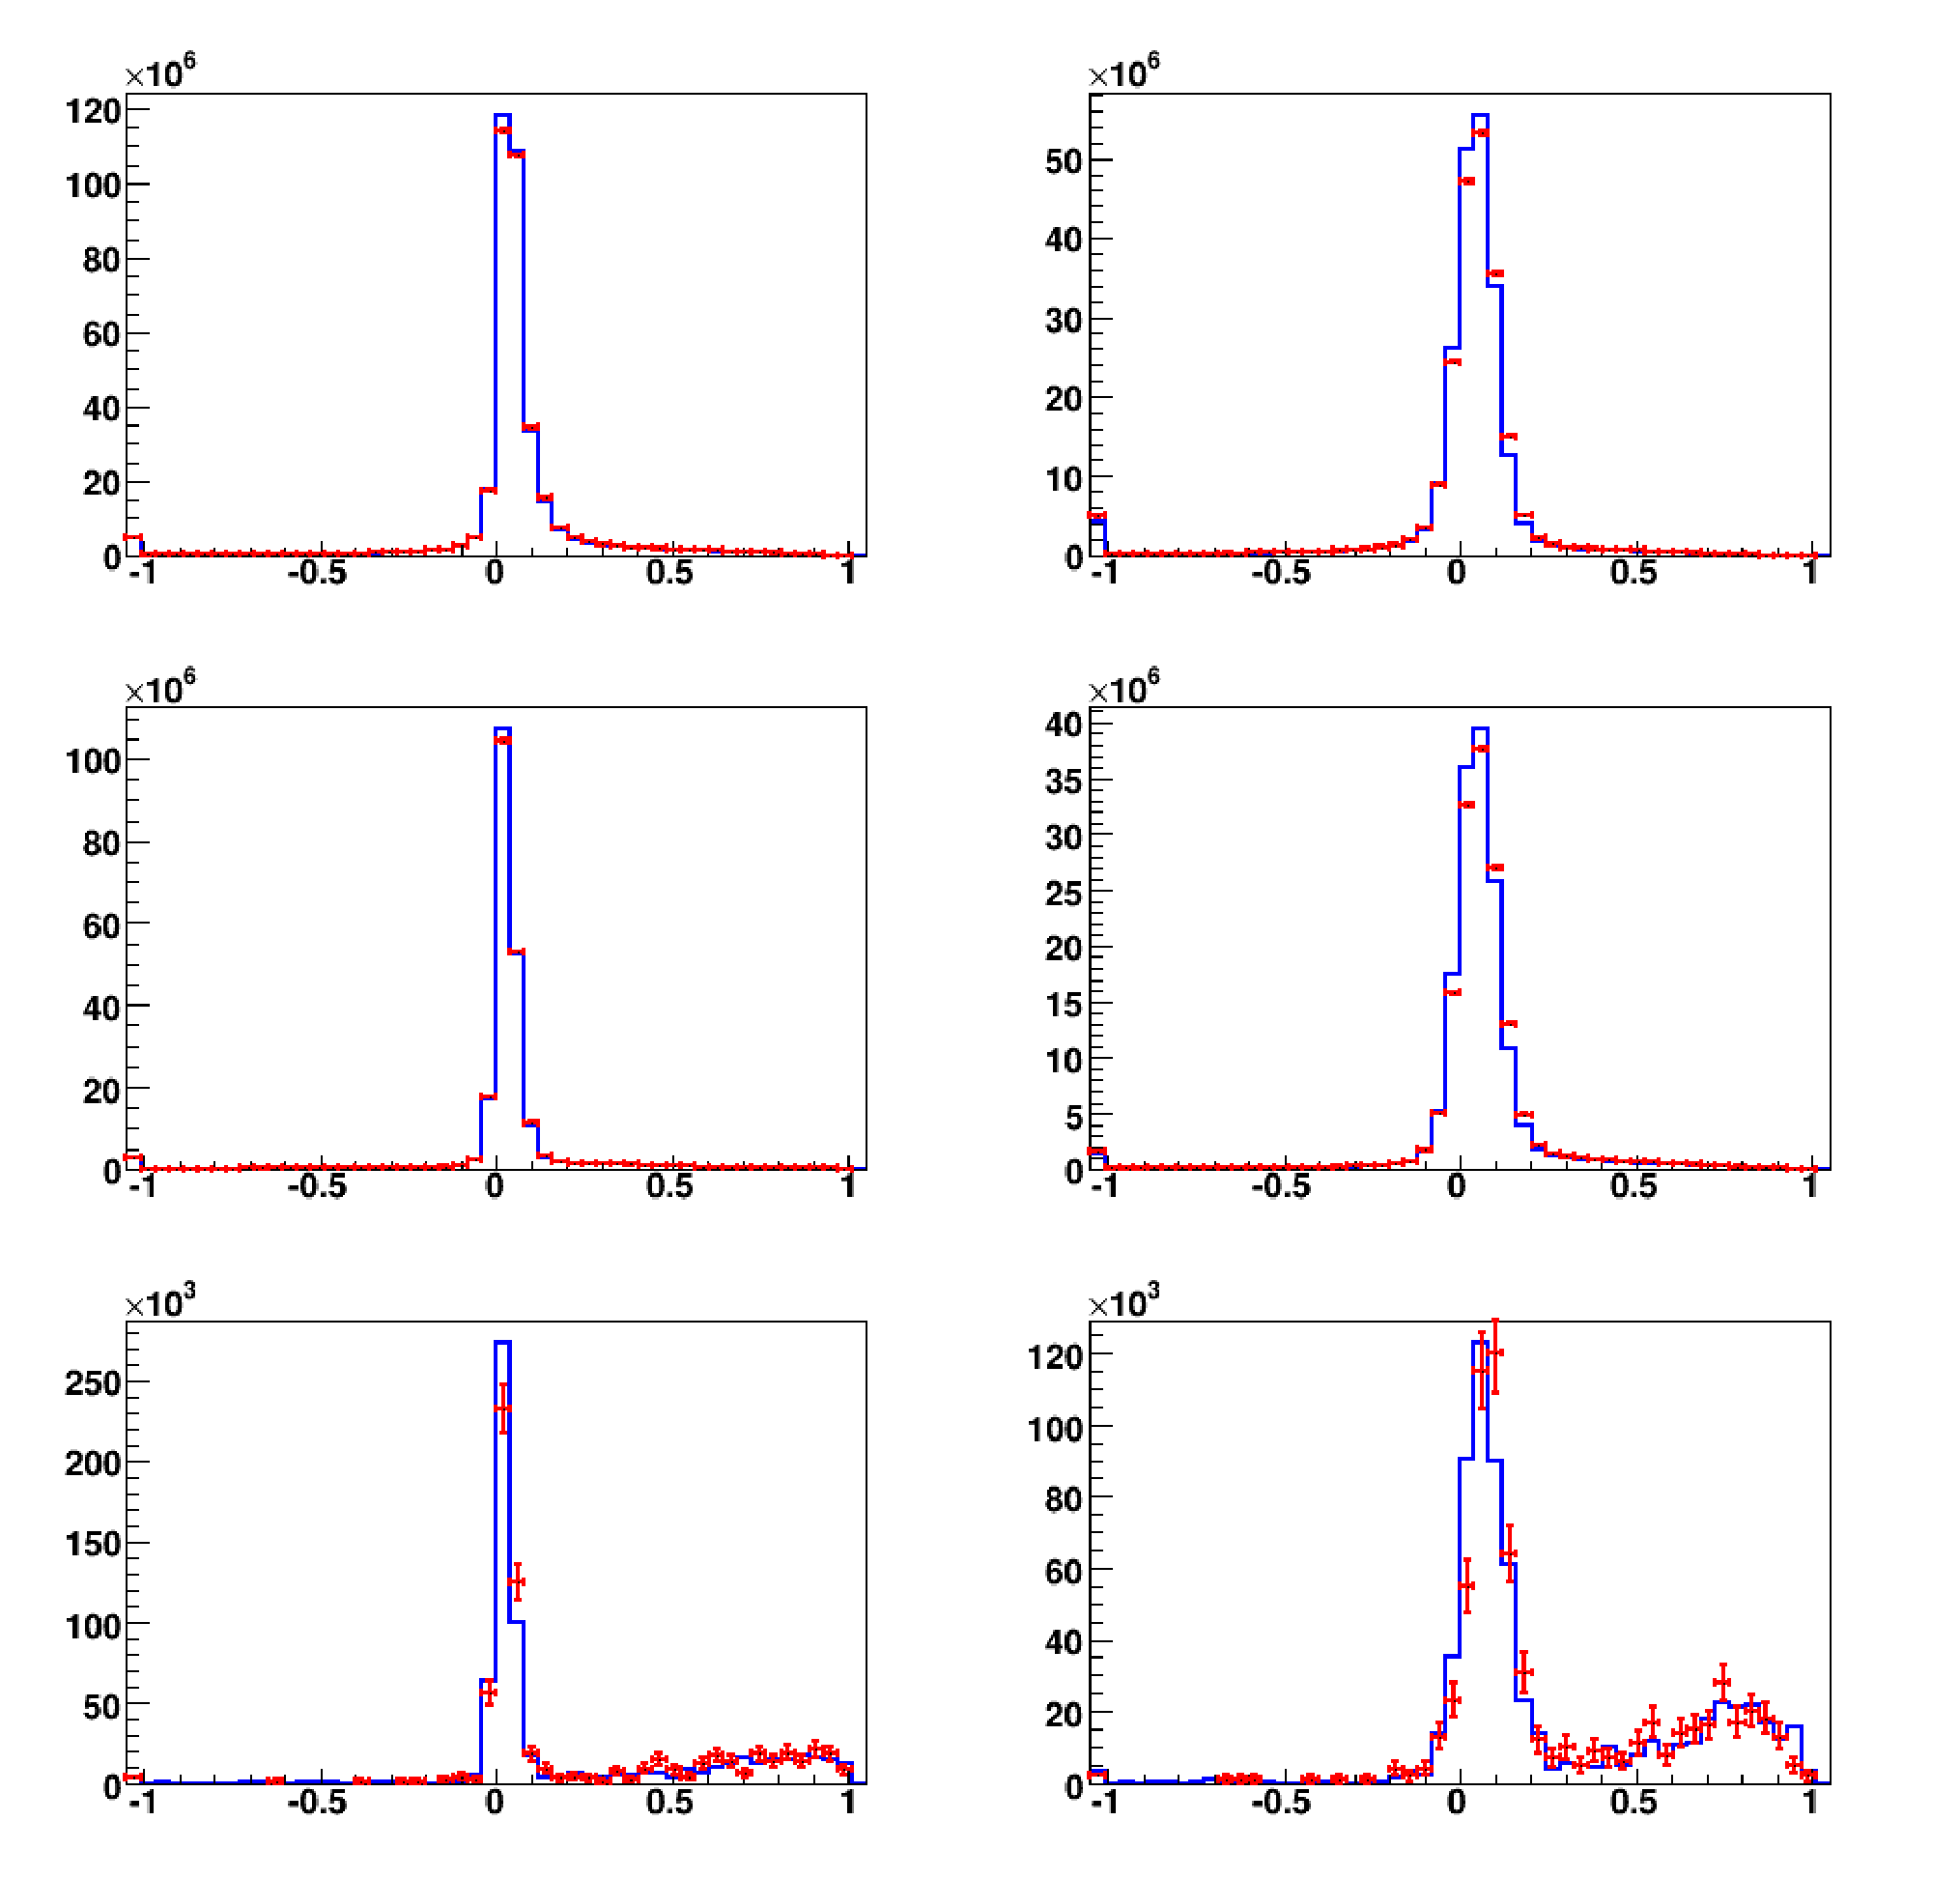
\includegraphics[width=1\textwidth]{Images/fbrem_vs_pt.eps}
    \caption {$\fbrem$ distribution in $\pt$ bins for data (points) and MC (histogram). From the top to the bottom the $\pt$  bins are defined as: $\pt < 1 \GeVc$, $1< \pt < 5 \GeVc$,$\pt > 5 \GeVc$. Each row shows the distribution for Barrel (left) and Endcap (right).}
    \label{fig:fbrem in pt bins}
  \end{center}
\end{figure}

\begin{figure}
  \begin{center}
    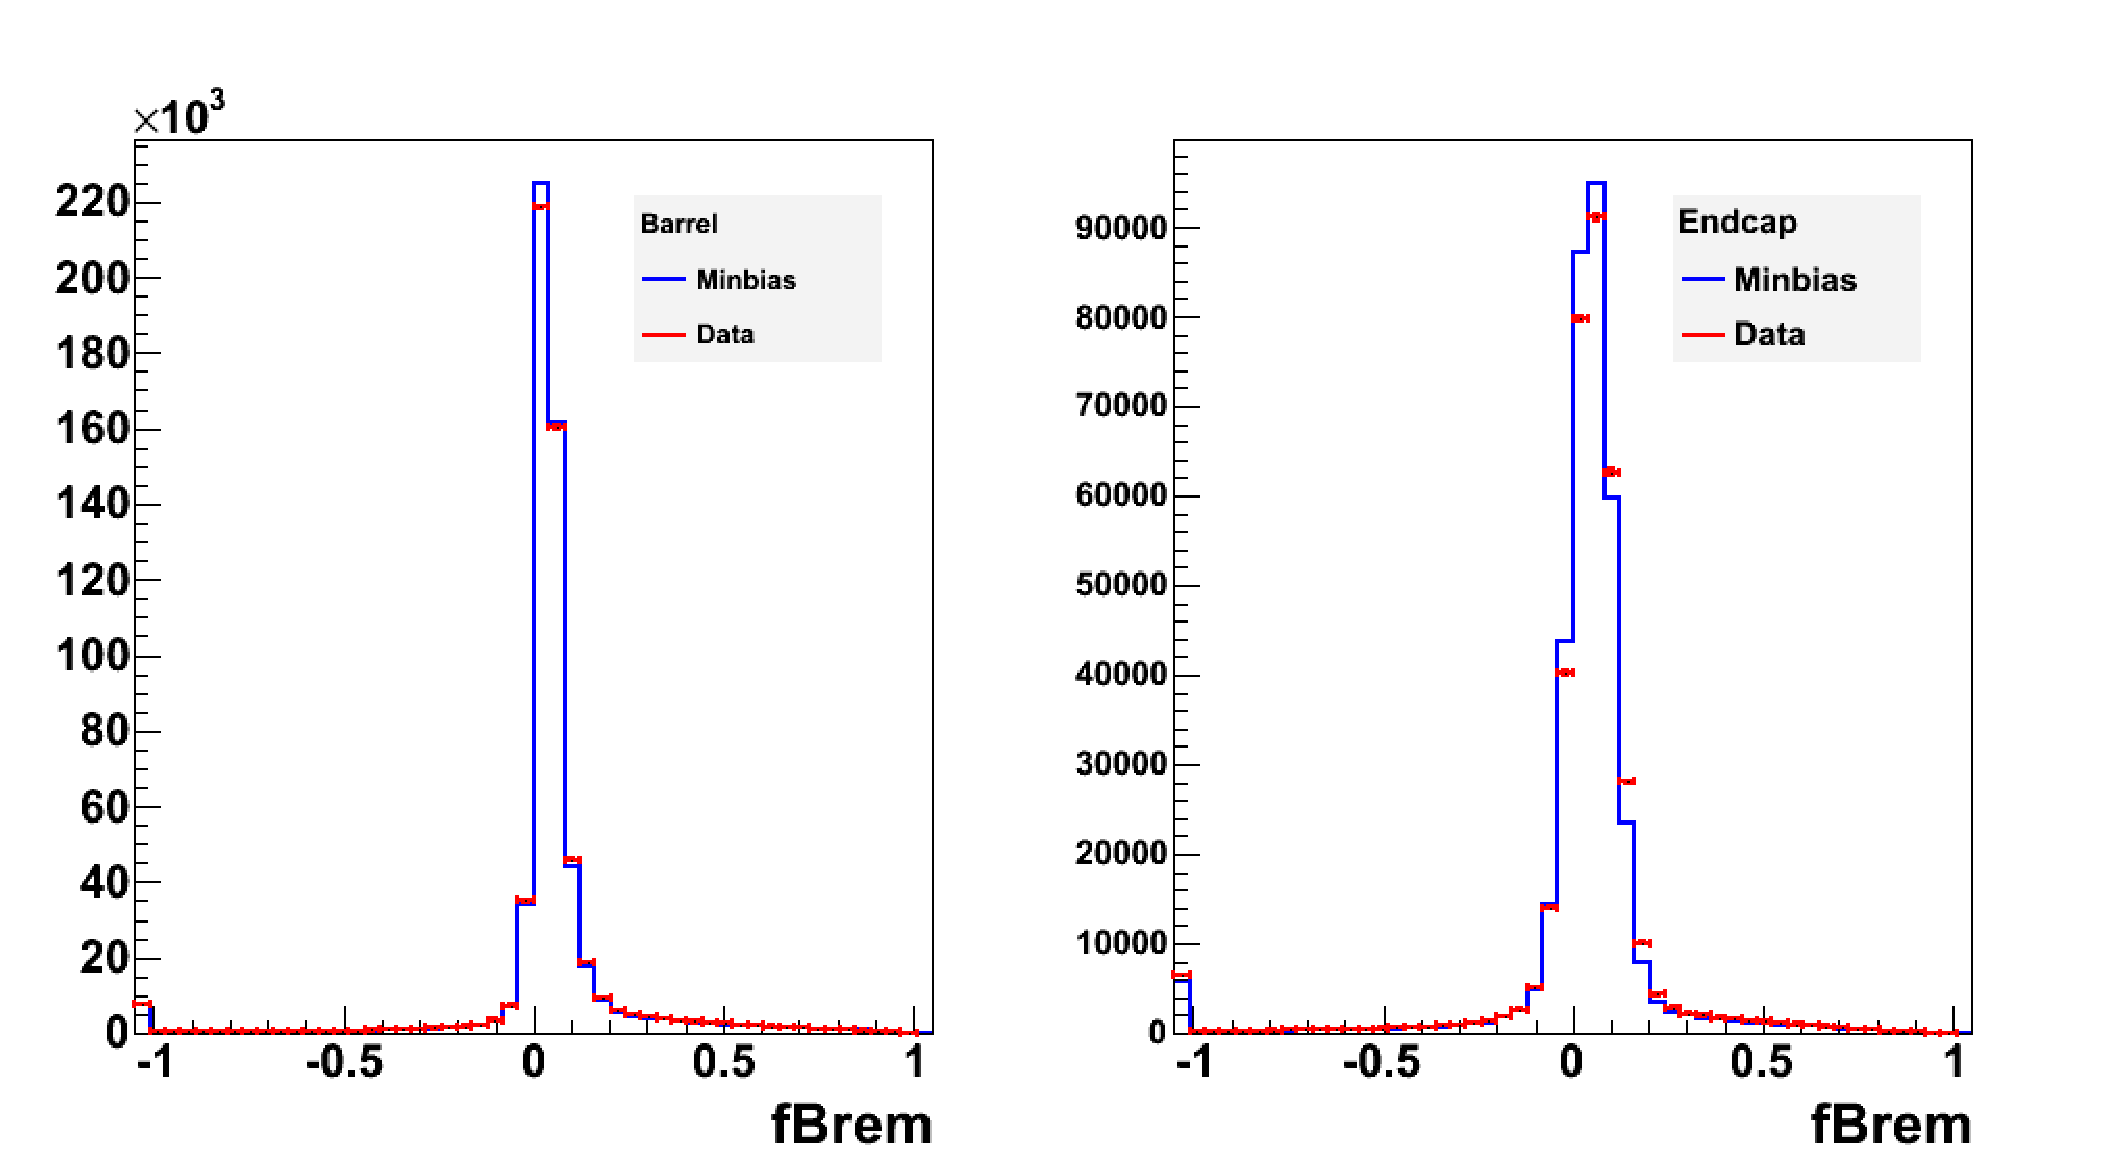
\includegraphics[width=.8\textwidth]{Images/fbrem_tot.eps}
    \caption{Total $\fbrem$ distribution for high purity GSF Tracks in data (points) and MC (histogram). The two plots show Barrel (left) and Endcap (right) distributions.}
    \label{fig:fbrem tot}
  \end{center}
\end{figure}

Another important variable related to GSF tracks that is used in the Electron Identification selection
is the number of missing hits. This is the number of crossed layers without compatible hits
in the back-propagation of the track to the beam-line.
Fig.~\ref{fig:mssinghits} shows the missing hits variable comparison in Barrel and Endcap. The distributions
show some discrepancies that need to be understood.

\begin{figure}
  \begin{center}
    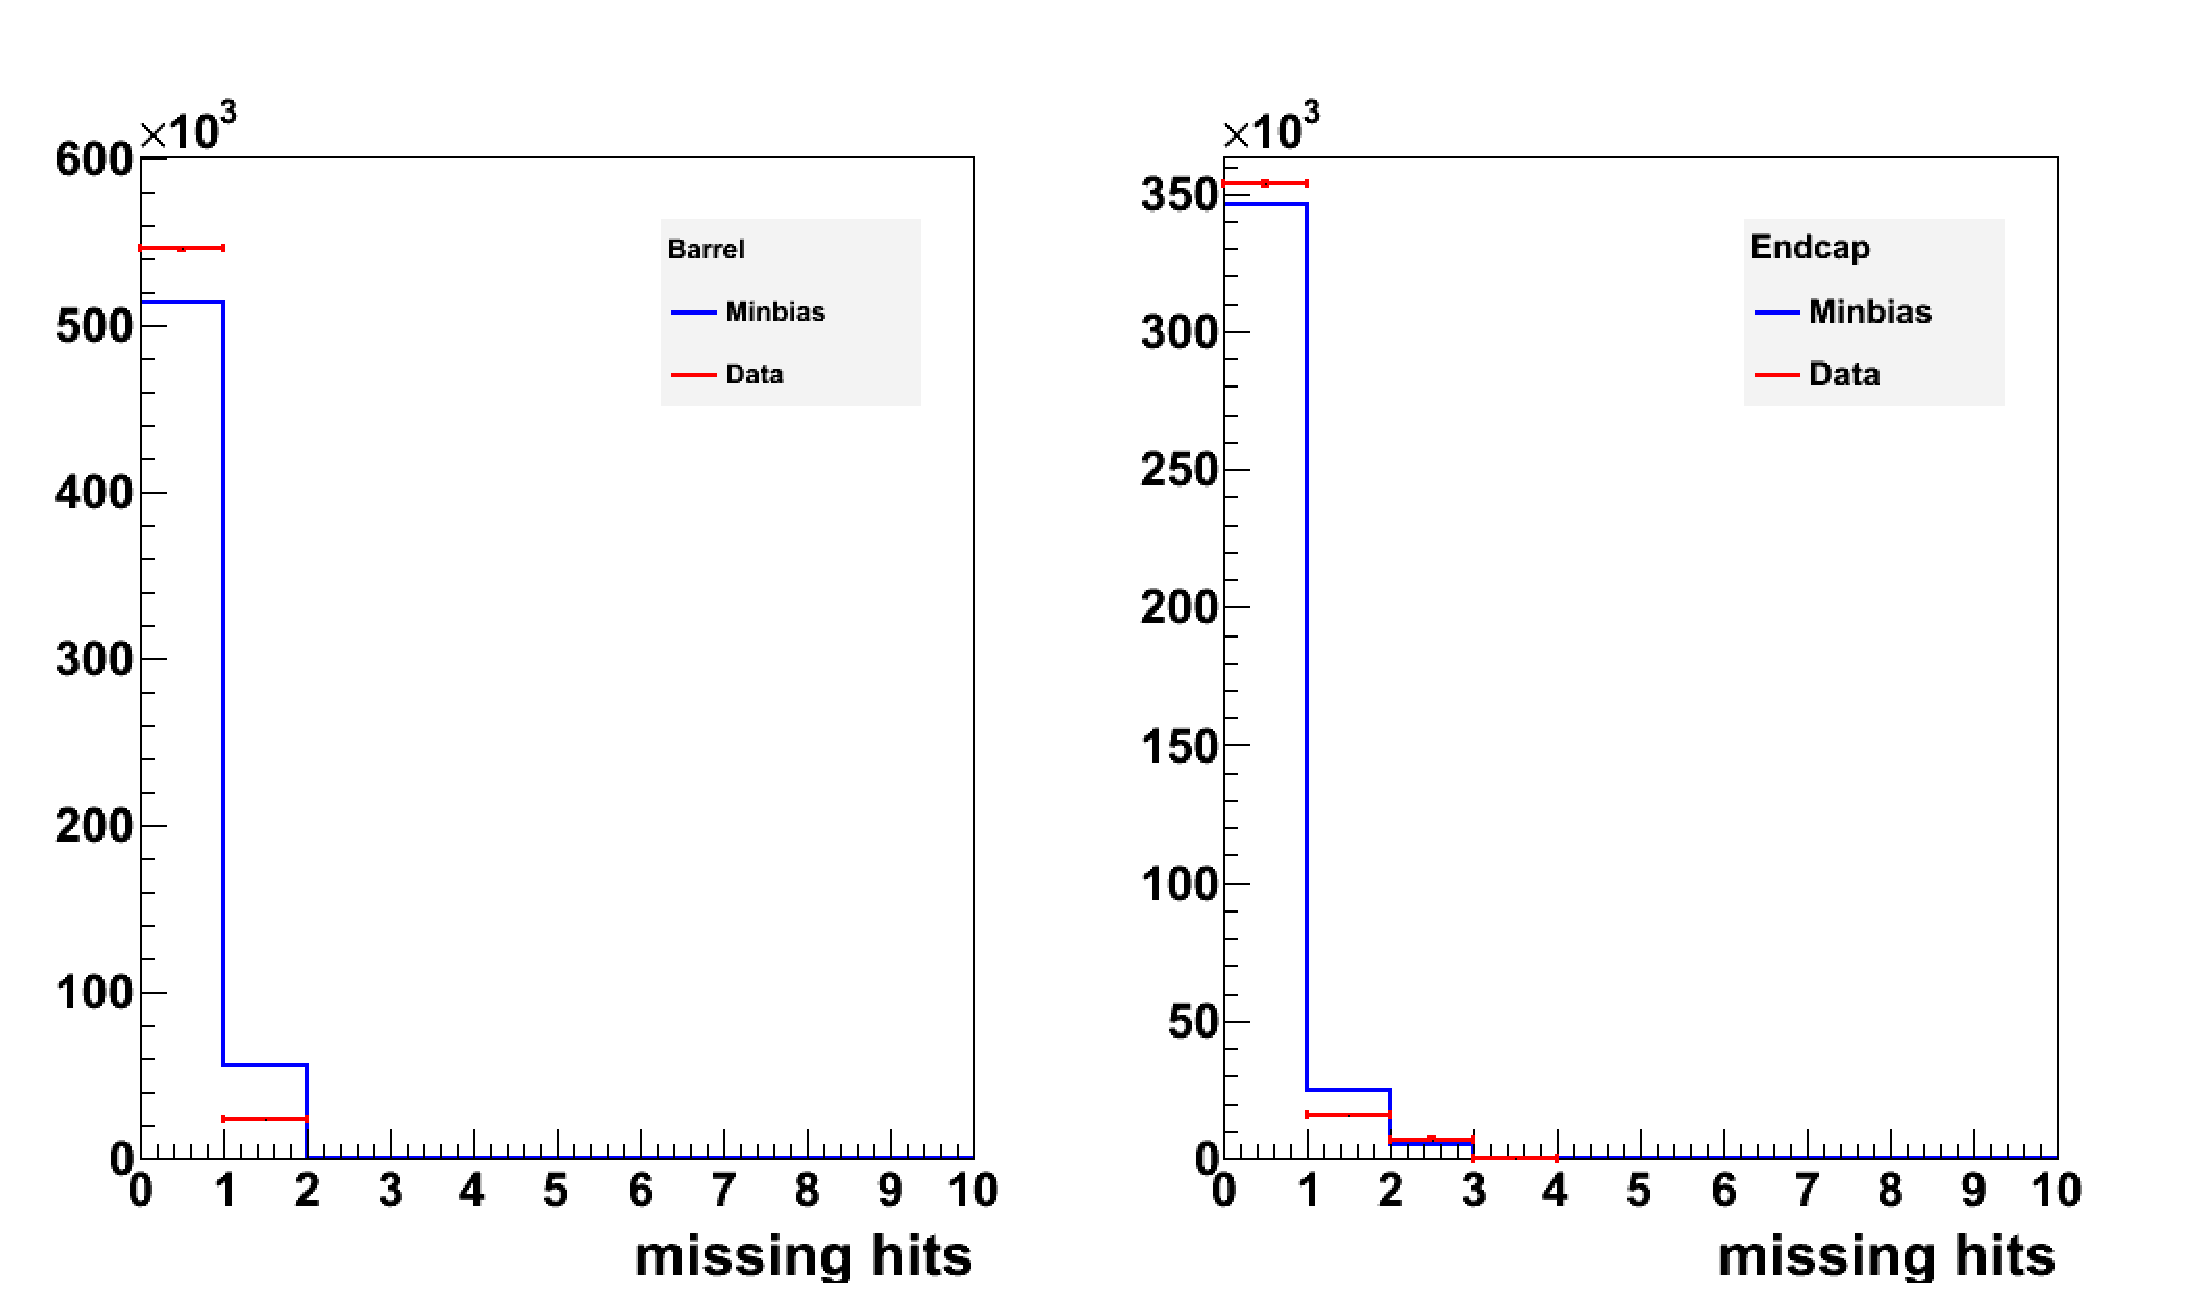
\includegraphics[width=.8\textwidth]{Images/gsf_mishits.eps}
    \caption {Missing hits distribution for high purity GSF Tracks in data (points) and MC (histogram). The two plots show the distributions in Barrel (left) and Endcap (right).}
    \label{fig:mssinghits}
  \end{center}
\end{figure}

Electron Identification selection uses also an Impact Parameter cut (computed with respect to the 
reconstructed vertex).
Fig.~\ref{fig:ip} shows the impact parameter distributions which is in good agreement with MC except
for the dip around 0.5 cm which is under investigation.

\begin{figure}
  \begin{center}
    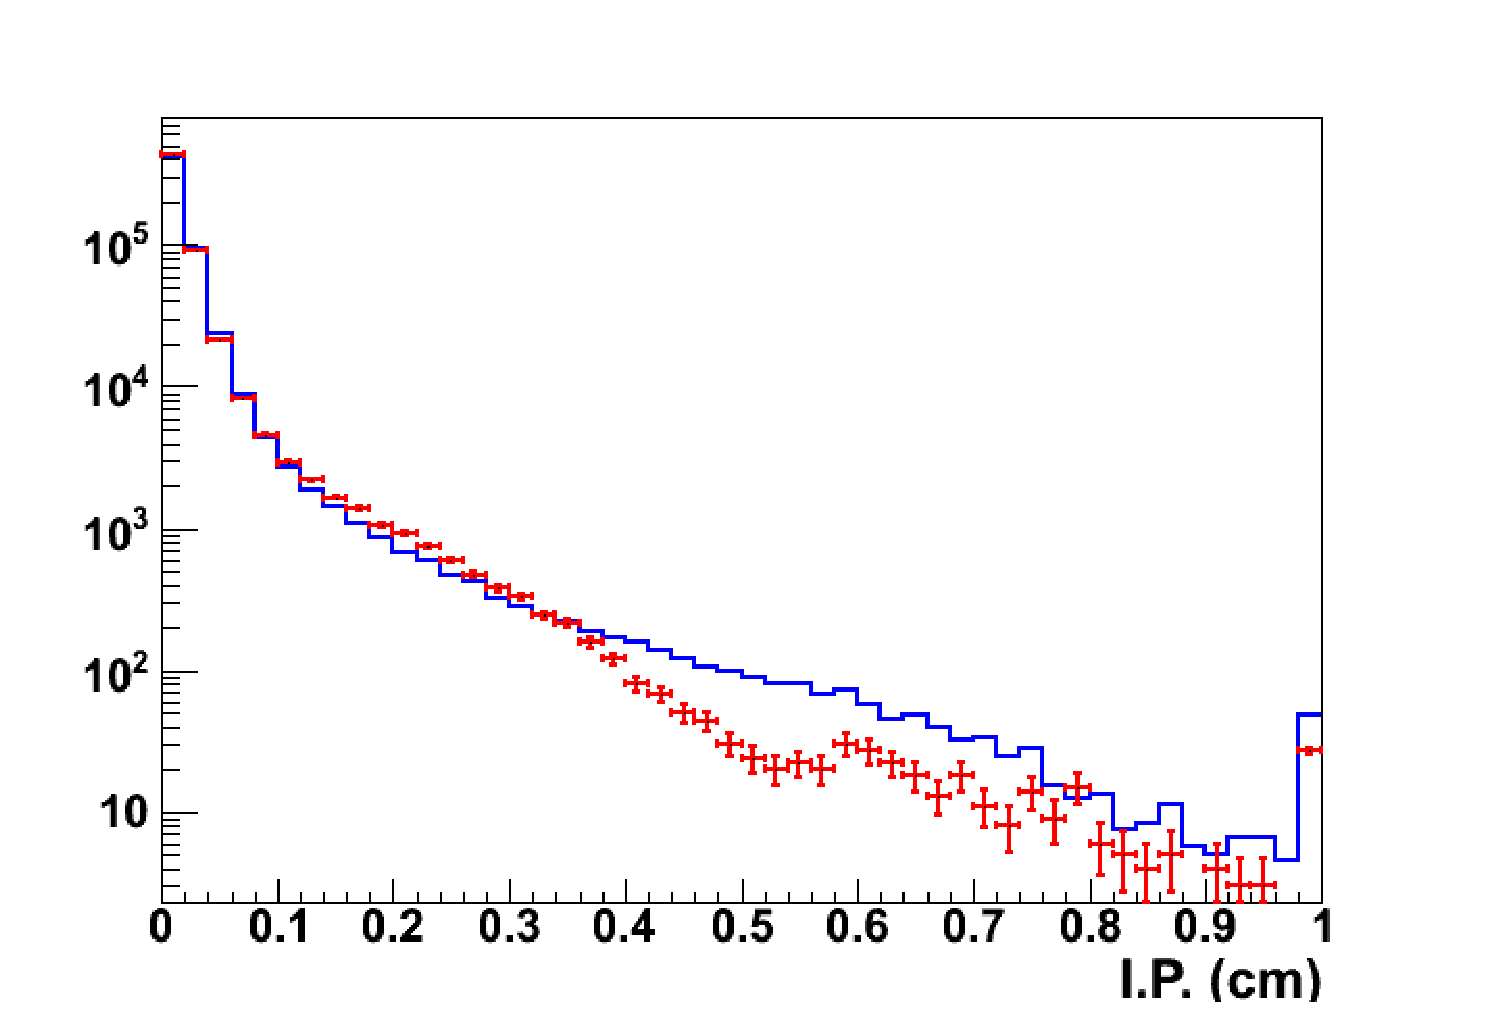
\includegraphics[width=0.6\textwidth]{Images/gsf_ip.eps}
    \caption {Impact parameter computed with respect to the reconstructed vertex of high purity GSF Tracks in data (points) and MC (histogram).}
    \label{fig:ip}
  \end{center}
\end{figure}

Other GSF tracks distributions have been checked even if not directly correlated with Electron Identification selection. 
Fig.~\ref{fig:chi2} shows the $\chi^{2}$ of the GSF Tracks in Barrel and Endcap which is very well reproduced by the MC simulation.
Also ratio between the track momentum estimations of the GSF (mode) and of the associated 
CTF track are well reproduced, the distributions for Barrel and Endcap are shown in Fig.~\ref{fig:pin over p}.

We have also compared the number of hits per track for a GSF track and
the corresponding CTF. 
The variable that has been studied is the ratio of the number of hits of GSF and CTF tracks
(nhits(GSF)/nhits(CTF))
and it has been done in four bins of the ratio $\pout/\pin$ of the GSF track. 
It turns out that the four distributions are in good agreement with the simulation. Beside that it
is clear how the ratio of number of hits increases as the fraction $\pout/\pin$ decreases: the higher
is the energy loss in the Tracker the harder is for the CTF pattern
recognition to produce a track as long as for the GSF one.
Fig.~\ref{fig:nhits} shows the four distributions.

\begin{figure}
  \begin{center}
    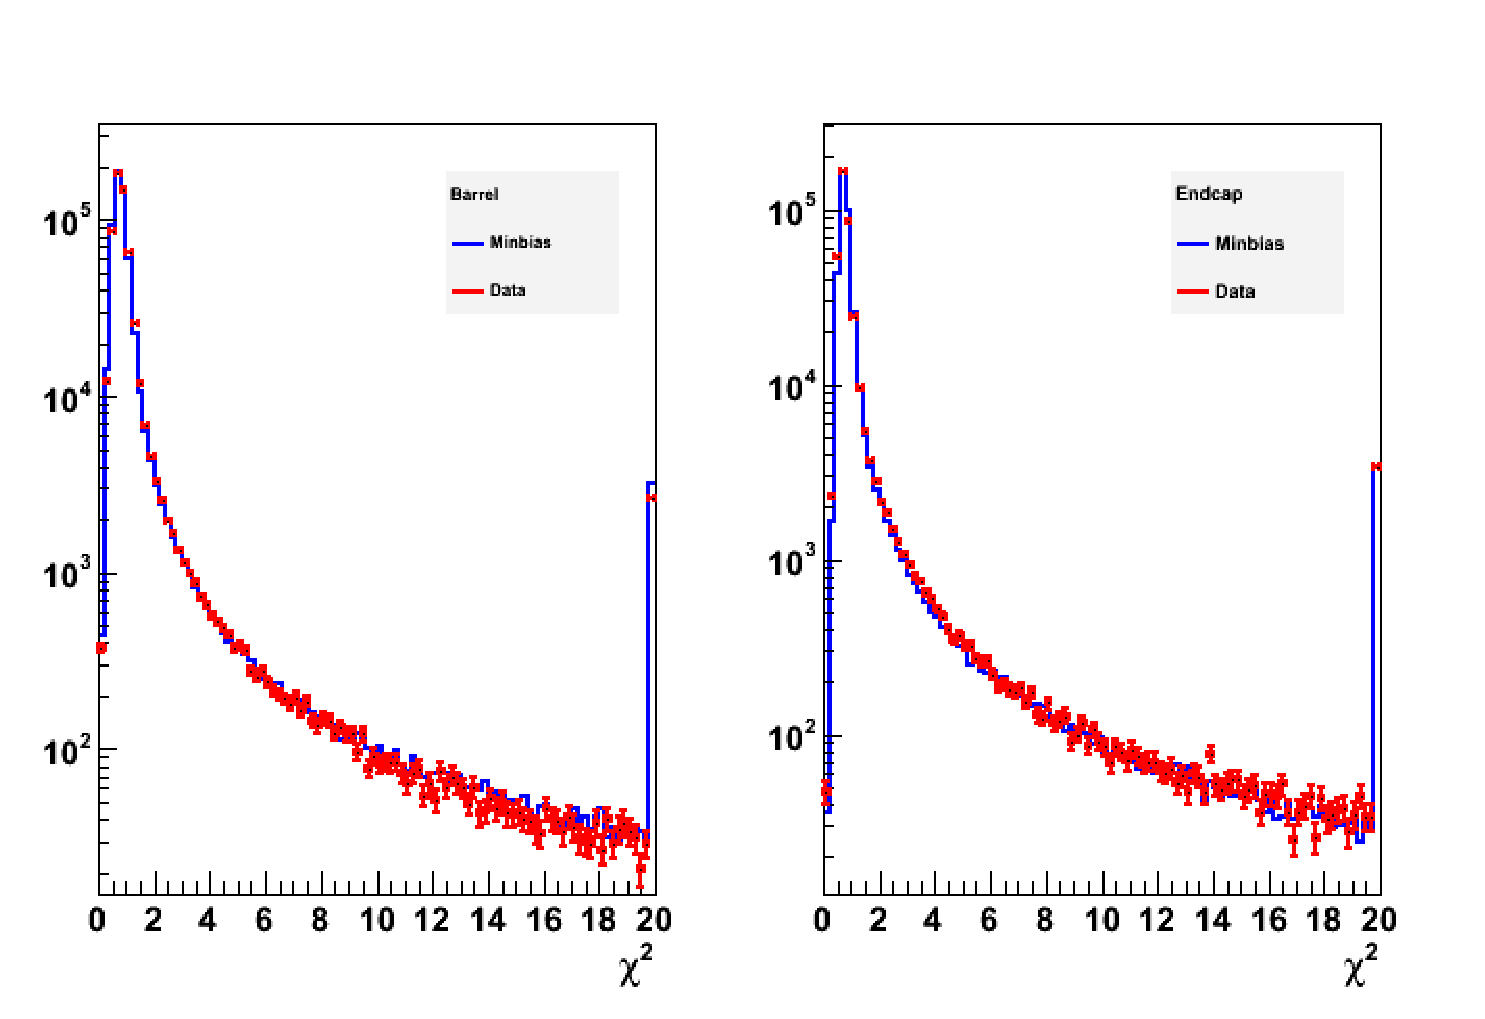
\includegraphics[width=.8\textwidth]{Images/gsf_chi2.eps}
    \caption {$\chi^{2}$ distribution for high purity GSF Tracks in data (points) and MC (histogram). The two plots show the distributions in Barrel (left) and Endcap (right).}
    \label{fig:chi2}
  \end{center}
\end{figure}

\begin{figure}
  \begin{center}
    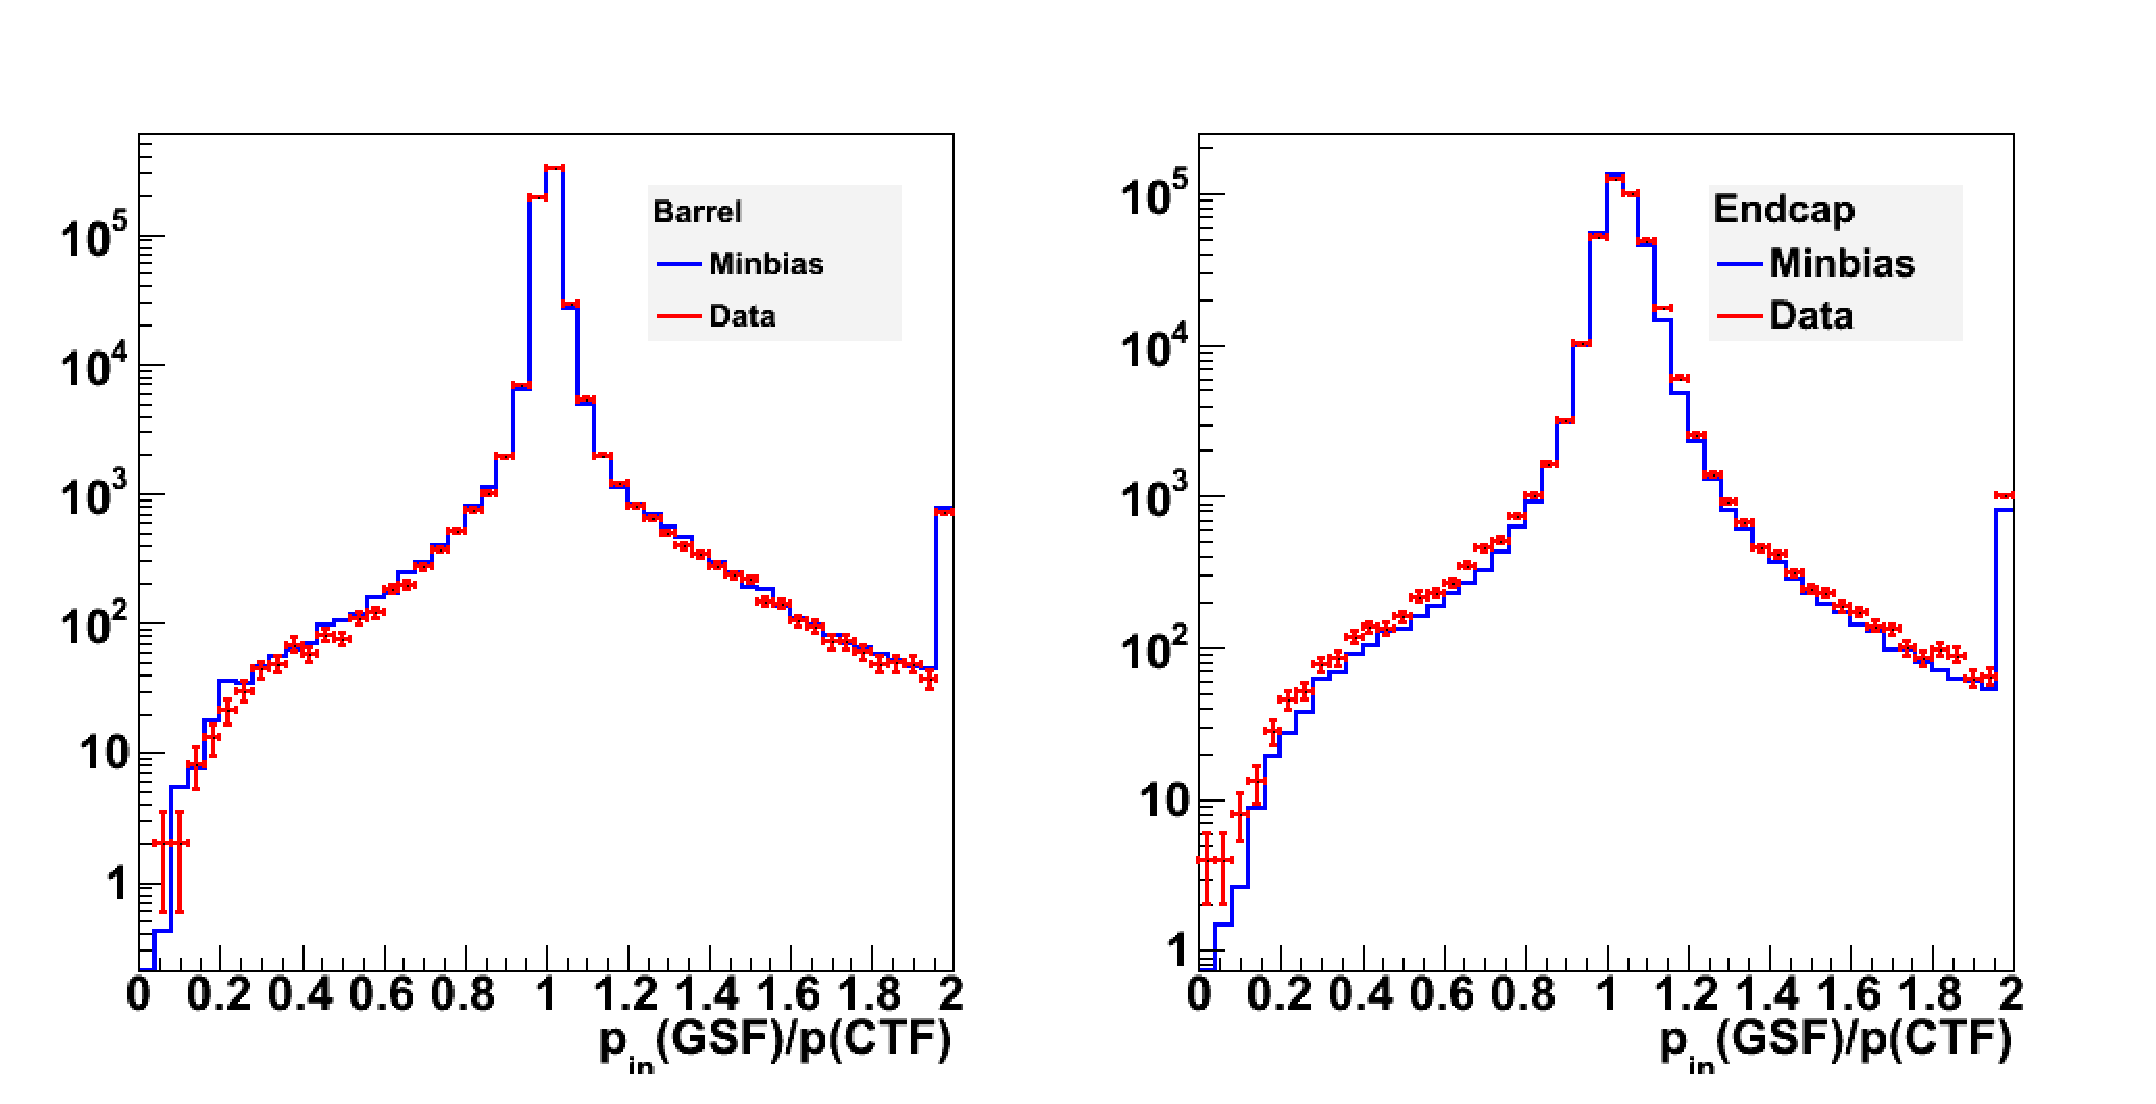
\includegraphics[width=.8\textwidth]{Images/pin_over_p.eps}
    \caption {Ratio between the $\pin$ momentum estimated as the mode of the GSF Track and the momentum of the associated CTF track. Data are in points, MC in histogram.  The two plots show the distributions in Barrel (left) and Endcap (right).}
    \label{fig:pin over p}
  \end{center}
\end{figure}

\begin{figure}
  \begin{center}
    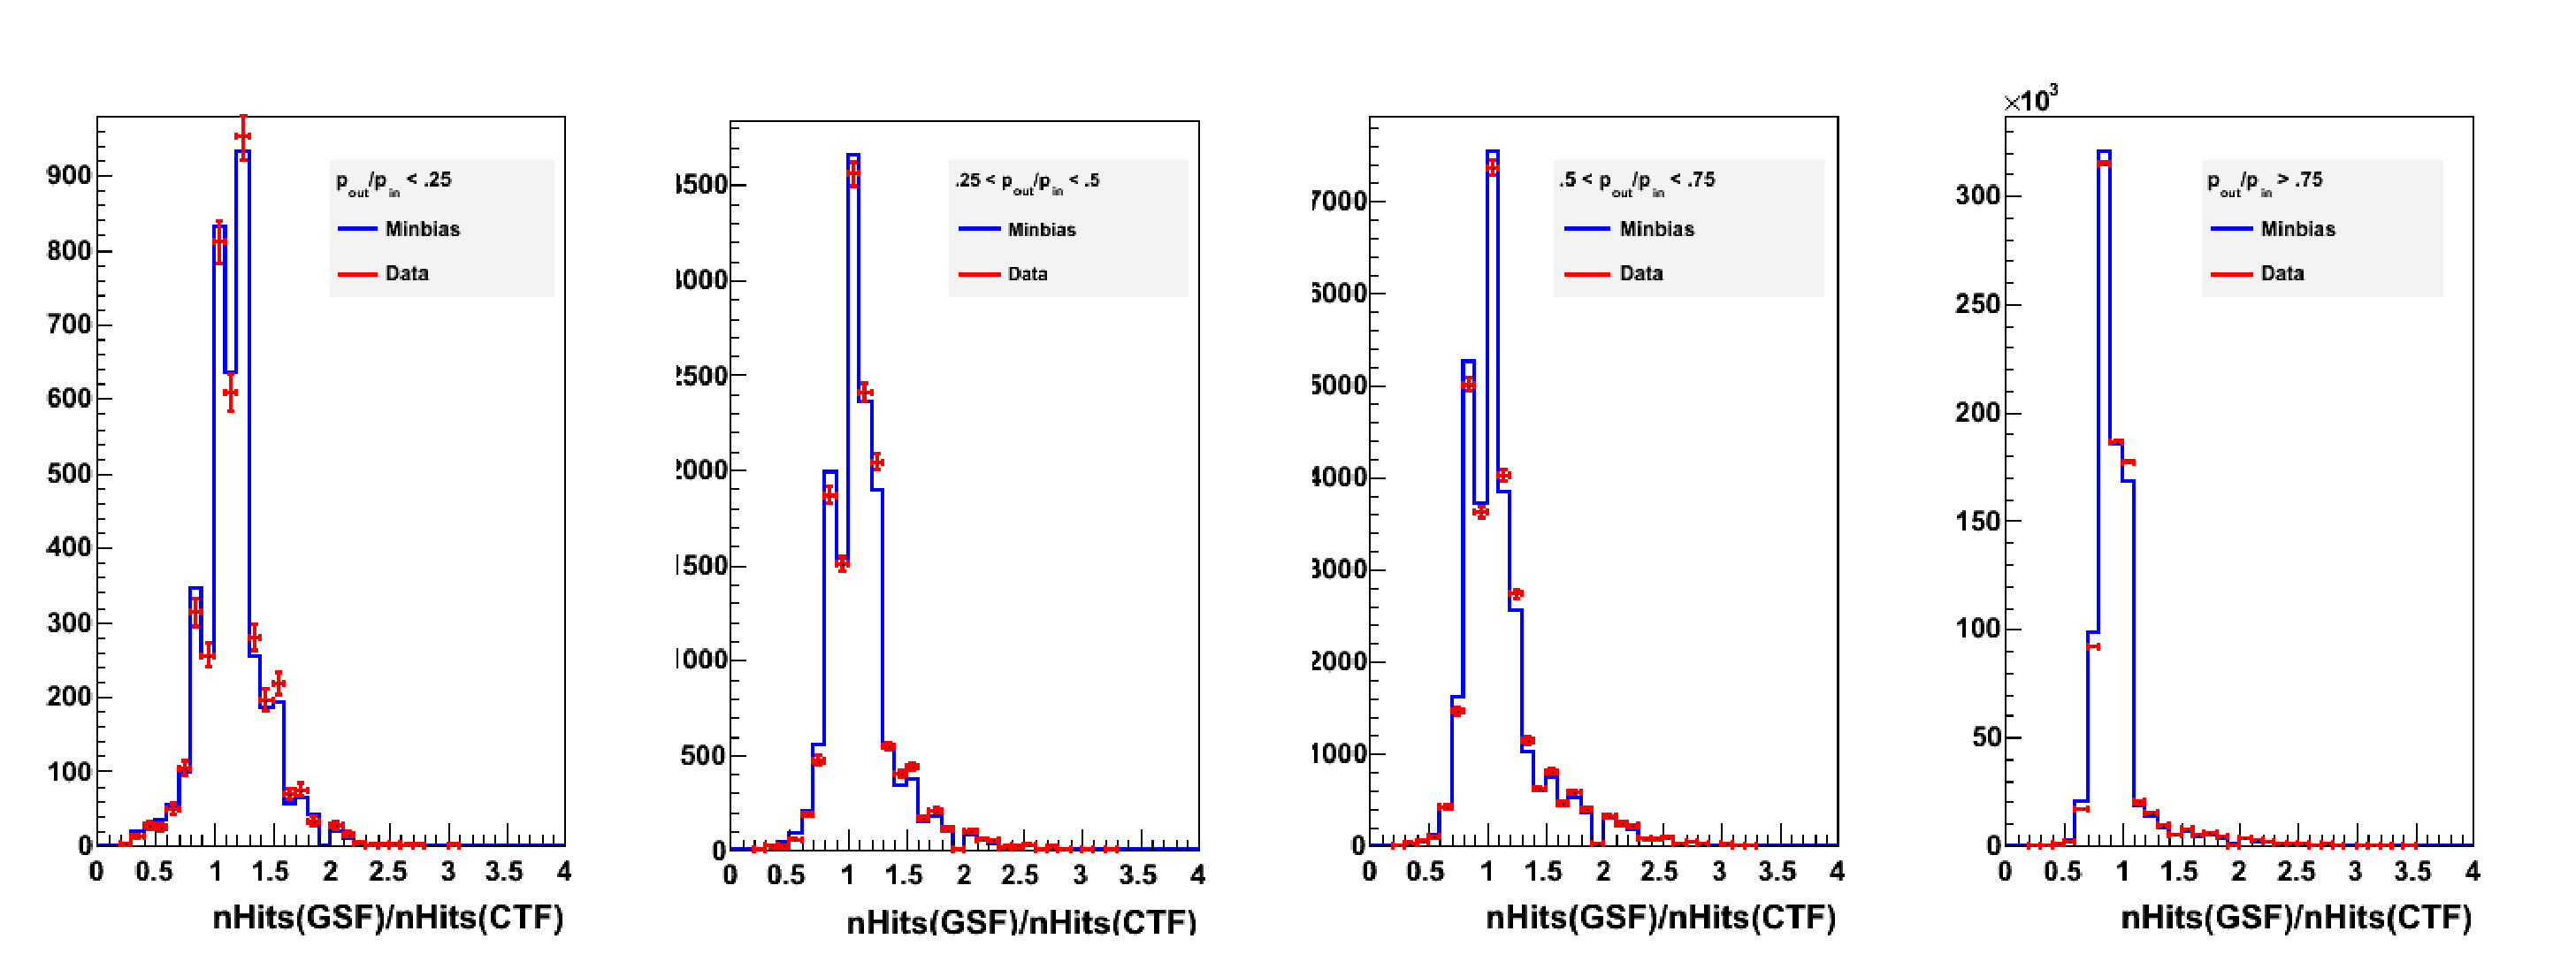
\includegraphics[width=1\textwidth]{Images/frac_nhits.eps}
    \caption {Ratio between number of hits of high purity GSF Tracks and the associated CTF Track in data (points) and MC (histogram). The distributions are shown in bins of the fraction $f = \pout$/$\pin$, from left to right: $f<.25$, $.25<f<.5$, $.5 < f<.75$, $f>.75$.}
    \label{fig:nhits}
  \end{center}
\end{figure}

\section{Conclusions}
In the process of commissioning the Category Based Electron Identification selection we wanted
to check the reliability of pure tracking variables, like $\fbrem$ and missing hits, comparing
collision data recorded during December 2009 data taking and MC simulated minimum bias events.
Unfortunately the number of electron candidates reconstructed during 2009 data taking was not 
enough. To increase the available statistic we have performed a full re-reconstruction using 
GSF Tracking algorithm starting from the seed collection used in the general CTF tracking.
All the studied variables show a quite good agreement between the collision data and the simulation 
even if more investigations are needed to understand the remaining discrepancies.


\pagebreak

%\begin{thebibliography} {99}
%\bibliographystyle{unsrt}
%\bibitem{bib:cmsnote_2006_040}
%S. Baffioni {\it et al.}, ``Electron Reconstruction in CMS'',
%{}The European Physical Journal C, {\bf 49} (2007) 1099-1116
%%CMS NOTE-2006/040.
%\bibitem{bib:cmsanote_2009_164}
%F. Beaudette {\it et al.}, ``Electron Reconstruction in CMS''
%CMS AN-2009/164.
%\bibitem{bib:cmsanote_2008_082}
%J. Branson {\it et al.}, ``A cut based method for electron identification in CMS'' 
%CMS AN-2008/082.
%\bibitem{bib:cmsanote_2008_110}
%E. Di Marco {\it et al.}, ``Electron Identification in the CMS experiment based on a likelihood algorithm'' 
%CMS AN-2008/110.
%\bibitem{bib:cmsanote_2005_065}
%S. Baffioni {\it et al.}, ``Electron Selection and Identification in CMS'',
%CMS AN-2005/065.
%\bibitem{bib:cmsanote_2009_108}
%G. Daskalakis {\it et al.}, ``Data driven selection cut tuning for electrons''
%CMS AN-2009/108.
%\bibitem{bib:pas_ewk_2009_004}
%The CMS Collaboration,
%``W and Z production in the electron channel at sqrts = 10 TeV''
%CMS PAS EWK-2009-004.
%\bibitem{SISCONE} G. P. Salam and G. Soyez, ``A practical Seedless Infrared-Safe Cone jet algorithm'', 
%JHEP 05 (2007) 086, [arXiv:0704.0292].
%\bibitem{splots} 
% M.~Pivk and F.~R.~Le Diberder, 
% %``SPlot: A statistical tool to unfold  data distributions,'' 
% Nucl.\ Instrum.\ Meth.\ A {\bf 555} (2005) 356
% [arXiv:physics/0402083].  
% %%CITATION = NUIMA,A555,356;%%
%\bibitem{bib:PFT2009_001}
%The CMS Collaboration, 
%``Particle-Flow Event reconstruction in CMS and Performance for Jets, Taus, and $E_T^{miss}$ '', 
%CMS PAS PFT-09/001.
%\bibitem{bib:PFT2009_006}
%The CMS Collaboration, ``Electron reconstruction within the Particle Flow Algorithm'', 
%CMS PAS PFT-09/006 (in preparation).
%\bibitem{bib:heepIDNote} 
%O. Charaf {\it et al.}, ``Electron ID at High Energies'', 
%CMS AN-2008/045.
%\bibitem{bib:heepTwiki} 
%Electron ID and Isolation for high energy electron: \emph{https://twiki.cern.ch/twiki/bin/view/CMS/HEEPELectronID}
%\bibitem{bib:AN_2009-159} 
%W. Andrews {\it et al.}, ``Study of Photon Conversion Rejection'', 
%CMS AN-2009/159.
%\end{thebibliography}
%
%\input{Conclusions/Appendix.tex}

\end{document}

